\documentclass[12pt,a4paper,openright,twoside]{book}
\usepackage[utf8]{inputenc}
\usepackage{disi-thesis}
\usepackage{code-lstlistings}
\usepackage{notes}
\usepackage{shortcuts}
\usepackage{acronym}
\usepackage{float}

% Information used in the title page
\school{\unibo}
\programme{Corso di Laurea in Ingegneria e Scienze Informatiche}
\title{Utilizzo di Neverlang per la modellazione di Domain Specific Languages\note{TODO: chiedere conferma titolo}} %Utilizzo di Neverlang per l'implementazione di un DSL SQL-like
\author{Terenzi Mirco}
\date{\today}
\subject{Programmazione ad Oggetti}
\supervisor{Prof. Viroli Mirko}
\cosupervisor{Prof. Aguzzi Gianluca}
\academicyear{2023-2024}

% Definition of acronyms
\acrodef{FOP}{Feature-Oriented Programming}
\acrodef{OOP}{Object-Oriented Programming}
\acrodef{DSL}{Domain-Specific Language}
\acrodef{JVM}{Java Virtual Machine}
\acrodef{AST}{Abstract Syntax Tree}
\acrodef{CFG}{Context-Free Grammar}
\acrodef{SQL}{Structured Query Language}

\mainlinespacing{1.241} % line spacing in mainmatter, comment to default (1)

\begin{document}

\frontmatter\frontispiece
\begin{abstract}
%TODO
\end{abstract}


\tableofcontents   
\listoffigures
%\lstlistoflistings

\mainmatter
%----------------------------------------------------------------------------------------
\chapter{Introduzione} %TODO
\label{chap:introduzione}
%----------------------------------------------------------------------------------------

\paragraph{Struttura della Tesi} %TODO

%----------------------------------------------------------------------------------------
\chapter{Contesto}
\label{chap:contesto}
%----------------------------------------------------------------------------------------

\section{Domain-Specific Languages}
In modo del tutto opposto rispetto ai linguaggi general-purpose, progettati per poter essere utilizzati in ogni contesto con un’efficienza e 
un grado d’espressività relativamente uguali, i \ac{DSL} sono ottimizzati per uno specifico ambito e risultano essere, in molti casi, una 
soluzione molto più naturale rispetto a quella fornita dai primi \cite{Hudak1997}. Tra gli esempi più comuni di \ac{DSL} troviamo SQL, LaTeX 
(utilizzato anche per la scrittura di questo documento) e CSS.

Nonostante la definizione di \ac{DSL} sia chiara, non è altrettanto immediato definire se un linguaggio sia o meno un \ac{DSL}. In questo caso, 
vi sono alcuni principi chiave da osservare \cite{Fowler2010}:
\begin{itemize}
    \item Un \ac{DSL} è un linguaggio di programmazione e, come tale, la sua struttura dovrebbe essere progettata in modo da essere facile da 
    comprendere per gli esseri umani e, al tempo stesso, eseguibile da un calcolatore.
    \item Essendo un linguaggio, deve avere un senso di fluidità e la sua espressività deve essere derivata non solo da un’espressione 
    individuale, ma anche dalla combinazione di più istruzioni.
    \item Coerentemente alla definizione, un \ac{DSL} dovrebbe implementare l'insieme minimo di caratteristiche necessarie per poter supportare 
    il dominio applicativo di interesse ed evitare funzioni non fondamentali che potrebbero rendere il linguaggio più difficile, 
    sia da utilizzare sia da comprendere.
\end{itemize}

L’utilizzo di questa tipologia di linguaggi di programmazione comporta una serie di vantaggi:
\begin{itemize}
    \item \textbf{Produttività}: Essendo il livello d’astrazione maggiore, di conseguenza, lo è anche la produttività. Questo perché è 
    possibile utilizzare direttamente i concetti propri del dominio applicativo, non essendo limitati dalla necessità di mantenere una 
    generalità atta ad ottenere un linguaggio applicabile in molteplici contesti  \cite{Kelly2008}. Come indicato da Paul Hudak 
    \cite{Hudak1997} ed illustrato nella \cref{fig:sw-dev-cost}, assumendo che il costo di sviluppo di un programma sia lineare, possiamo 
    ipotizzare che il costo iniziale richiesto sia maggiore nel caso si utilizzasse un \ac{DSL} rispetto a metodologie più convenzionali 
    (considerando il caso in cui il linguaggio andasse sviluppato, se ne venisse utilizzato uno esistente tale costo sarebbe significativamente 
    minore). Ciò nonostante, la pendenza della curva è considerevolmente più bassa e quindi, da un determinato punto in poi, l’utilizzo di 
    \ac{DSL} porterebbe un risparmio significativo.
    \begin{figure}[H]
        \centering
        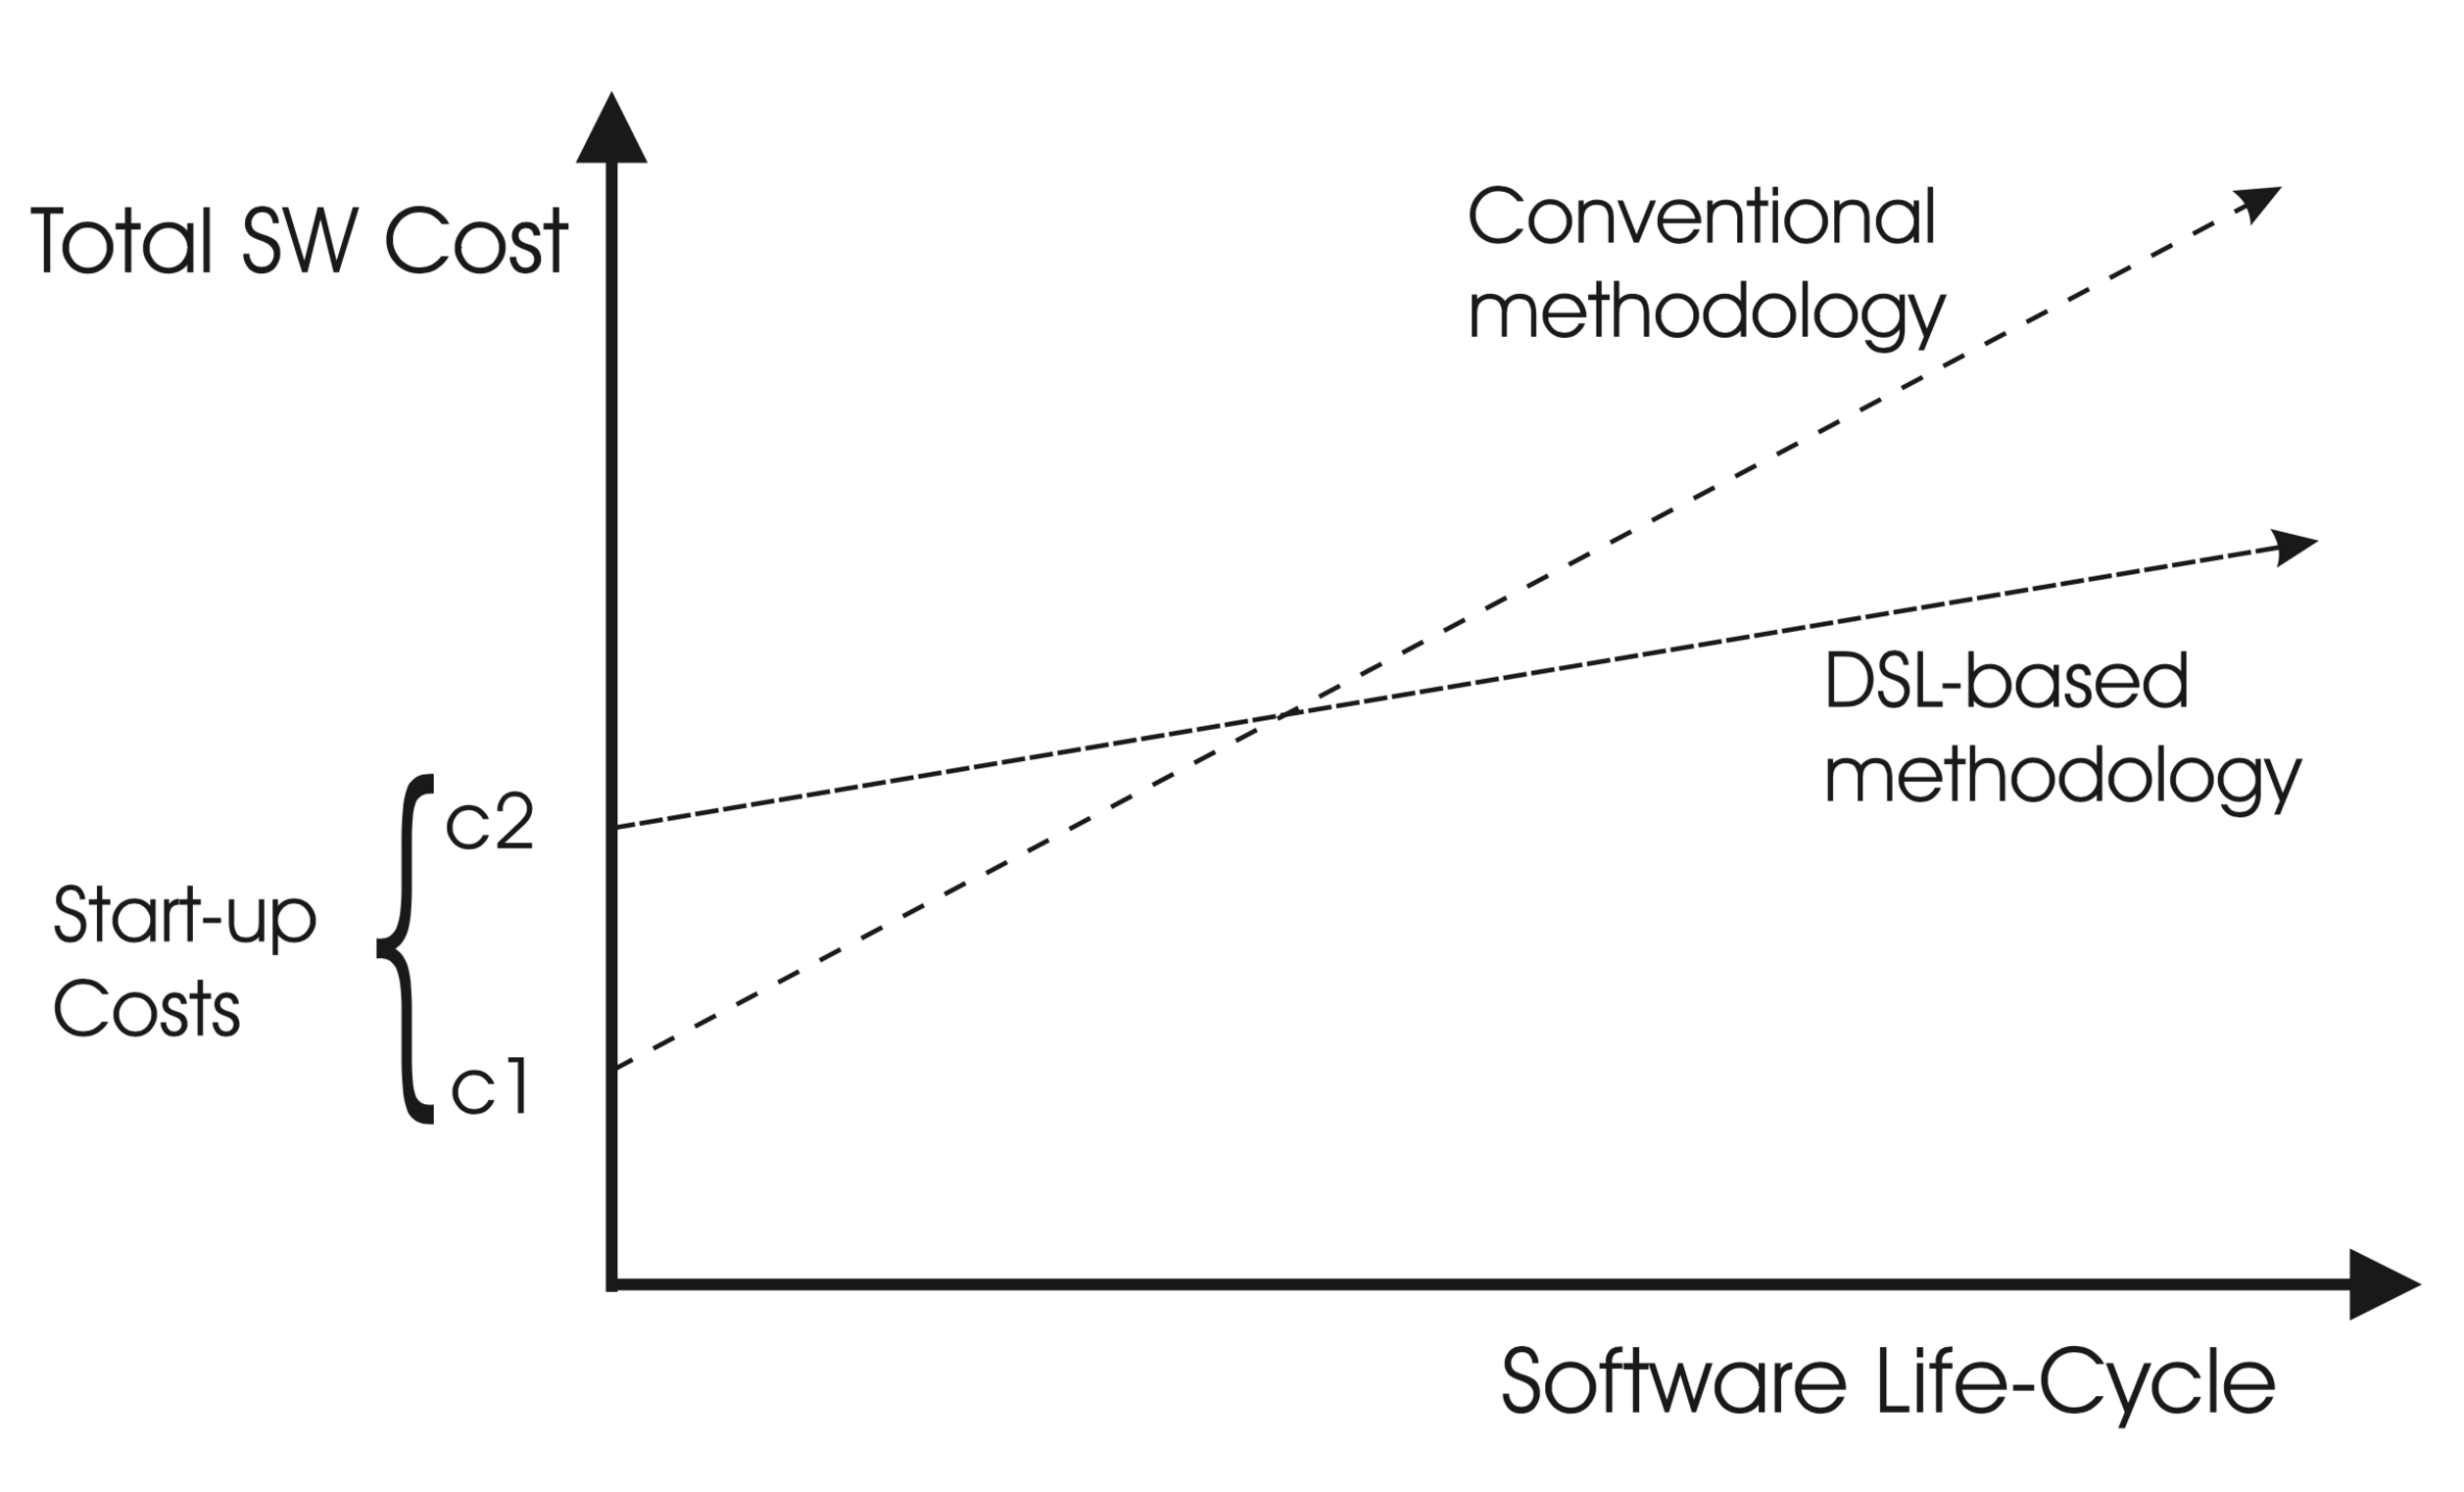
\includegraphics[width=.8\linewidth]{figures/sw-dev-cost.pdf}
        \caption{Grafico rappresentante il costo di sviluppo di un software in funzione del tempo, confrontando l'utilizzo di un DSL con 
        quello di un linguaggio general-purpose.}
        \label{fig:sw-dev-cost}
    \end{figure}
    \item \textbf{Qualità del codice}: L'utilizzo di \ac{DSL} favorisce anche una migliore qualità del codice. Infatti, il linguaggio può 
    includere regole direttamente trasposte dal dominio all'interno del quale è applicato. In questo modo risulta molto più difficile, talvolta 
    impossibile, ottenere dei risultati non attesi. Ad esempio, Antti Raunio, capo ingegnere del progetto EADS \cite{EADS}, afferma che ``la 
    qualità del codice generato è chiaramente migliore [...] perché il linguaggio di modellazione è stato progettato per adattarsi 
    all'architettura del nostro terminale''\footnote{Di seguito riportata l'affermazione citata, in lingua originale:``the quality of the 
    generated code is clearly better, simply because the modelling language was designed to fit our terminal architecture''}. Inoltre, 
    l'offuscamento della reale complessità del problema, dovuto all'utilizzo di \ac{DSL}, consente ai nuovi sviluppatori di lavorare ad un 
    alto livello d'astrazione, senza dover conoscere tutti i dettagli inerenti all'implementazione del linguaggio \cite{EADS}. 
    \item \textbf{Migliore manutenibilità}: Sebbene l'uso di \ac{DSL} non renda l'implementazione necessariamente meno complessa di quanto 
    si possa ottenere utilizzando un linguaggio \textit{general-purpose}, la manutenibilità del codice risulta essere accentuata %TODO: è corretto "accentuata"?
    \cite{Klint2010}.  Infatti, considerando il volume del codice, l'utilizzo di \ac{DSL} comporta una minor quantità di codice da comprendere, 
    facilitandone la modifica. Inoltre, è possibile  ignorare il problema di mantenere coerente ciò che è definito dalla grammatica con la 
    struttura gerarchica definita dall'\ac{AST} in quanto quest'ultimo si evolve con la prima \cite{Brabrand2010}.
\end{itemize}

\section{Grammatica non contestuale}
Nel campo dell’informatica, una grammatica formale è costituita da regole che descrivono precisamente come vengono generati i simboli di un 
linguaggio formale, partendo da un insieme finito chiamato alfabeto. Ogni regola sintattica, detta anche produzione, è espressa nella forma 
$A \rightarrow x$, dove $A$ è un simbolo non terminale e $x$ è una combinazione di simboli terminali e/o non terminali.

In particolare, la grammatica non contestuale, o \ac{CFG}, è un tipo specifico di grammatica formale che deriva il proprio nome dal fatto che 
le regole sintattiche mantengono la loro validità indipendentemente dai simboli che precedono o seguono il simbolo non terminale a cui si 
applicano. Questa caratteristica è dovuta al fatto che le regole sintattiche di una grammatica non contestuale ammettono soltanto una variabile 
non terminale sul lato sinistro della regola \cite{Linz2022}.

Le grammatiche non contestuali assumono un ruolo fondamentale nella teoria dei linguaggi formali, in particolare nella definizione e nell’analisi 
dei linguaggi di programmazione. La \ac{CFG} è utilizzata principalmente per la modellazione della sintassi, ma viene impiegata anche nella 
costruzione di interpreti e compilatori \cite{Linz2022}.

\section{Compilazione del codice}
Il compilatore è un software fondamentale nel campo della programmazione e dell’informatica, il cui compito è tradurre il codice sorgente 
(scritto in un linguaggio di alto livello) in un linguaggio di basso livello (tipicamente il linguaggio macchina o codice oggetto) che può 
essere eseguito 
dal calcolatore.

Il processo di compilazione è suddiviso in diverse fasi, ognuna delle quali ha un ruolo specifico nel convertire il codice sorgente in un 
programma eseguibile. Le fasi principali sono di seguito elencate \cite{Aho2006}:
\begin{itemize}
    \item \textbf{Analisi lessicale}: Durante la fase dell'analisi lessicale, talvolta definita anche \textit{scanning}, la sequenza di 
    caratteri di input viene analizzata e divisa in porzioni significative, chiamate lessemi. Per ogni lessema viene prodotto come output un 
    token, definito come coppia di valori \texttt{<nome-token, valore-attributo>}, che viene processato dalla fase successiva.
    \item \textbf{Analisi sintattica}: La fase dell'analisi sintattica, più comunemente indicata come \textit{parsing} (allo stesso modo, 
    il programma che svolge queste operazioni è chiamato \textit{parser}) o in italiano parsificazione, prevede che i token siano 
    utilizzati per creare una rappresentazione ad albero che descriva efficacemente la struttura grammaticale dell'input. Un esempio di 
    questo tipo di rappresentazione è costituito dall'albero sintattico. Al suo interno, ogni nodo rappresenta un'operazione e i nodi ad 
    esso discendenti, chiamati anche figli, rappresentano gli operandi dell'operazione definita dal primo. La parsificazione è svolta 
    principalmente secondo due metodologie \cite{Grune2006}:
    \begin{itemize}
        \item l’analisi \textbf{top-down} consiste nell'emulare il processo di produzione della frase. In questo modo, partendo dal simbolo 
        iniziale si procede per fasi ad evolvere l'output in modo da farlo corrispondere alla frase ottenuta come input. Il nome indica che 
        l'albero sintattico viene costruito partendo dall'alto, ossia dal nodo radice, proseguendo verso il basso;
        \item l’analisi \textbf{bottom-up}, al contrario, prevede di invertire il processo di produzione della frase, avendo come obiettivo 
        quello di ridurre la frase di input al simbolo iniziale.
    \end{itemize}
    \item \textbf{Analisi semantica}: In questo stadio della compilazione, il fine è analizzare la correttezza semantica del programma. Più 
    nello specifico, vengono utilizzati l'albero sintattico ottenuto dalla fase precedente e la tabella dei simboli per controllare che 
    l'input sia semanticamente coerente con quanto è definito dal linguaggio. Una parte fondamentale dell'analisi semantica è quella del 
    controllo del tipo (in inglese \textit{type-checking}), durante la quale il compilatore si accerta che il valore assegnato ad una 
    variabile sia ammissibile con il tipo di tale variabile e, allo stesso modo, che gli operandi utilizzati in un’operazione siano 
    compatibili con l’operazione stessa. Talora, le specifiche del linguaggio permettono delle conversioni di tipo chiamate coercizioni.
    \item \textbf{Generazione di codice intermedio}: Durante la compilazione, il compilatore genera una o più rappresentazioni intermedie. 
    L'albero sintattico precedentemente descritto rappresenta una delle varie forme che tali rappresentazioni possono assumere. In particolare, 
    devono essere rispettate due proprietà significative: le rappresentazioni devono essere facili da generare e facili da trasporre in codice 
    target (ossia il linguaggio di basso livello obiettivo della traduzione).
    \item \textbf{Ottimizzazione del codice}: Successivamente, si procede a perfezionare, per quanto possibile, il codice intermedio in modo 
    che si possa poi ottenere un codice finale migliore.
    \item \textbf{Generazione del codice}: Infine, il codice intermedio viene utilizzato per generare il codice target.
\end{itemize}

\section{Programmazione feature-oriented}
La programmazione orientata alle funzionalità, comunemente nota come \ac{FOP}, è un paradigma di programmazione focalizzato sulla modularizzazione 
del software. L’obiettivo principale della \ac{FOP} è facilitare la gestione e lo sviluppo di programmi complessi, consentendo ai programmatori 
di scomporli in unità modulari. Questa metodologia è ampiamente applicata in contesti di linee produttive di software e viene utilizzata per 
gestire la creazione di diverse versioni di un programma, adatte alle specifiche richieste dei clienti \cite{Apel2013}. Inoltre, la \ac{FOP} è 
impiegata per costruire sistemi configurabili, che prevedono l’attivazione o la disattivazione di funzionalità specifiche e offrono un elevato 
grado di personalizzazione.

Le caratteristiche principali della \ac{FOP} sono le seguenti:
\begin{itemize}
    \item \textbf{Riusabilità}: Confrontando la \ac{FOP} con l’approccio più classico della \ac{OOP} si nota come la prima offra una maggiore 
    modularità e flessibilità del codice. Di conseguenza, la riusabilità è amplificata poiché per ogni funzionalità implementata il nucleo 
    funzionale e la parte relativa alle interazioni sono mantenute separate \cite{Prehofer1997}.
    \item \textbf{Gestione della complessità}: La \ac{FOP} permette di gestire progetti di considerevole complessità grazie allo sviluppo 
    modulare del codice in unità distinte. Queste unità possono essere sviluppate e mantenute in modo indipendente, riducendo significativamente 
    l’interdipendenza e la complessità del sistema complessivo. Inoltre, la separazione delle funzionalità semplifica l’evoluzione del software, 
    poiché ogni modifica può essere limitata a una singola funzionalità senza influenzare l’intero sistema \cite{Prehofer1997}.
    \item \textbf{Adattabilità}: La \ac{FOP} consente una facile configurazione e personalizzazione dei sistemi software attraverso la selezione 
    e la composizione delle funzionalità. Questo approccio permette di creare diverse varianti di un prodotto software a seconda dei requisiti 
    specifici, facilitando l’adattamento a nuovi contesti o a esigenze mutate nel tempo \cite{Apel2013}.
\end{itemize}

\section{Neverlang}
Neverlang Language Workbench è un framework sviluppato presso l’Università di Milano dal professor Cazzola e dai suoi collaboratori, il cui scopo 
è favorire lo sviluppo di linguaggi di programmazione, in particolare seguendo il paradigma della \ac{FOP}.

È basato sull’idea che i linguaggi di programmazione abbiano un’intrinseca divisione modulare in più caratteristiche, o \textit{features}, ciascuna 
delle quali è implementata da un componente specifico. In accordo con tale visione, l’obiettivo del framework è definire i linguaggi tramite una 
divisione in frammenti, chiamati moduli, ognuno dei quali si occupa di implementare una specifica caratteristica e, infine, tramite la combinazione 
dei diversi moduli, ottenere un linguaggio di programmazione specifico per il contesto applicativo richiesto, ossia un \ac{DSL} 
\cite{NeverlangWebsite}.

Quando il codice viene compilato, ogni costrutto viene inserito in una rappresentazione chiamata \ac{AST}, o albero sintattico astratto. 
L'\ac{AST} è simile all'albero sintattico descritto in precedenza ma con la fondamentale differenza che non rappresenta ogni dettaglio della 
reale sintassi. È essenzialmente una versione alternativa e semplificata che consente di focalizzarsi sulla logica descritta dal linguaggio.

All’interno di ogni modulo vengono definite due parti principali:
\begin{itemize}
    \item la \textbf{sintassi}, utilizzando una grammatica formale non contestuale;
    \item la \textbf{semantica}, in funzione della sintassi e sfruttando i vari elementi non terminali e i loro attributi. Inoltre, il 
    comportamento del componente può essere suddiviso in diverse fasi, ciascuna definita da un ruolo specifico all'interno del modulo. Anche 
    l'ordine d'esecuzione dei ruoli può essere specificato e le tre tipologie di visite predefinite sono:
    \begin{itemize}
        \item Semi-automatica: Tale strategia prevede che i nodi siano visitati partendo dal nodo radice e discendendo ai nodi figli finché non 
        viene individuata una definizione semantica. Una volta trovata, il controllo della visita viene trasferito all'esecuzione di tale azione.
        \item \textit{Post-order}: In questo caso la visita dell'albero predilige la discesa in profondità, ciò significa che l'esecuzione delle 
        azioni definite dalla semantica dei vari nodi è posticipata a dopo che tutti i nodi figli sono stati valutati.
        \item Giustapposizione: Nei due metodi precedenti, ad ogni ruolo corrisponde una visita all'albero. Al contrario, quando due ruoli sono 
        giustapposti, la loro esecuzione viene eseguita ``in una volta'' e cioè tutte le azioni corrispondenti a tali ruoli sono eseguite in 
        sequenza in una singola visita all'albero.
    \end{itemize}
\end{itemize}

Successivamente, i componenti del linguaggio vengono definiti combinando definizioni di sintassi e semantica provenienti da diversi moduli 
all’interno di costrutti denominati \textit{slice}, ognuno dei quali contiene la definizione di un singolo componente del linguaggio. 
Infine, il linguaggio viene generato combinando i vari \textit{slice} insieme. \cite{Vacchi2015} 

Tra i vantaggi principali di Neverlang troviamo \cite{Cazzola2012}:
\begin{itemize}
    \item \textbf{Modularità}: Ognuno dei moduli che compongono il linguaggio viene compilato separatamente, permettendo di utilizzarne uno o 
    più di uno (in tal caso aggregandoli in uno \textit{slice}) all’interno di altri linguaggi.
    \item \textbf{Riutilizzo}: Neverlang offre la possibilità di riutilizzare frammenti di linguaggio in più di un contesto. Ad esempio, un 
    frammento può utilizzare la sintassi di un altro frammento definito in precedenza e ridefinirne la semantica, o viceversa. Inoltre, è 
    possibile ridefinire l’ordine dei simboli non terminali utilizzati nella sintassi o nella semantica importata.
    \item \textbf{Estensibilità}: L’architettura modulare utilizzata all’interno di Neverlang facilita l’estensione di linguaggi esistenti. 
    Per aggiungere nuove funzionalità non è necessario modificare il codice, ma è sufficiente integrare un nuovo \textit{slice}.
\end{itemize}


\section{Java}
In aggiunta a Neverlang, per la realizzazione del progetto è stato utilizzato Java. Java è un linguaggio di programmazione ad alto livello, 
orientato agli oggetti e a tipizzazione statica, sviluppato da Sun Microsystems nel 1991. È molto diffuso e ben supportato, con una vasta 
comunità di sviluppatori e una grande quantità di librerie. Uno degli obiettivi principali di Java è quello di essere il più possibile 
autonomo rispetto alla piattaforma di esecuzione, permettendo di scrivere una volta il codice e farlo eseguire su qualsiasi \ac{JVM}, 
indipendentemente dall'architettura del calcolatore \cite{IBMWebsite}.

Java è stato utilizzato per la realizzazione del progetto in quanto Neverlang è progettato per essere completamente integrato con esso. Il suo 
compilatore (nlgc) è stato sviluppato per poter convertire il codice scritto utilizzando il DSL di Neverlang in un nuovo codice supportato 
dalla \ac{JVM}. Inoltre, Neverlang permette di utilizzare Java (ma non solo; anche Scala, ad esempio, è supportato) come linguaggio per la 
definizione della semantica all'interno dei moduli del \ac{DSL}. Ciò è possibile in quanto gli accessi a variabili non terminali, definiti 
all'interno della sintassi, sono sostituiti dallo specifico plug-in con accessi alla reale rappresentazione interna del linguaggio. In 
particolare, l'accesso alle variabili viene effettuato tramite una chiamata all'n-esimo figlio dell'\ac{AST} \cite{Cazzola2013}.

%----------------------------------------------------------------------------------------
\chapter{Analisi e Requisiti}
\label{chap:requisiti}
%----------------------------------------------------------------------------------------

\section{Obiettivi}
Il progetto si propone di ricreare la sintassi e la logica di \ac{SQL} all’interno di un \ac{DSL} implementato utilizzando il framework 
Neverlang Language Workbench. L’obiettivo principale è modellare il linguaggio seguendo un approccio incrementale ed implementando le varie 
funzionalità in modo tale che possano essere aggiunte o rimosse dal progetto in modo indipendente.

Il linguaggio deve semplificare la gestione di un ampio quantitativo di dati e favorirne la manipolazione tramite le operazioni 
sviluppate al suo interno. Lo scopo è aiutare l’utente finale ad estrarre le informazioni di cui ha bisogno a partire dai dati già in suo 
possesso. Per raggiungere questo obiettivo, il programma deve implementare una serie di procedimenti necessari per la creazione, la modifica e 
l’eliminazione di tabelle, all’interno delle quali sono memorizzati i dati. Inoltre, è necessario gestire l’inserimento di tali dati, nonché 
la loro eventuale alterazione od eliminazione. Infine, il linguaggio dovrà fornire le operazioni richieste per selezionare, manipolare ed 
aggregare l’insieme di informazioni presenti nel database.

\section{Requisiti funzionali}
\label{sec:requisiti-funzionali}
Il \ac{DSL} dovrà implementare un insieme di caratteristiche tipiche di \ac{SQL}. Di seguito vengono elencate 
le principali:
\begin{itemize}
    \item \textbf{Gestione delle tabelle}: Per modellare la base di dati secondo le proprie esigenze, l’utente ha a disposizione una serie 
    di operazioni per creare o modificare le tabelle all’interno del database:

    \begin{itemize}
        \item La funzione \texttt{CREATE TABLE} permette di creare una nuova tabella e di specificare le colonne che la compongono. Ciascuna 
        colonna può avere vincoli sui dati che conterrà. Ad esempio, il vincolo espresso di default durante la fase di creazione della 
        tabella riguarda il tipo dei dati inseriti in ogni colonna, il quale dovrà essere coerente con quanto specificato nella definizione 
        della tabella. In aggiunta, è possibile indicare altre caratteristiche che il dato inserito dovrà rispettare, come l’unicità (ossia 
        che non sia uguale a un altro dato già presente nella tabella), la non nullità (l’informazione non può essere omessa) oppure la 
        definizione dell’attributo come chiave della tabella, comprendendo i vincoli di unicità e non nullità precedentemente descritti.
        \item L’operazione \texttt{ALTER TABLE} permette di modificare le tabelle già presenti nel database. Quando tale costrutto viene 
        utilizzato, è necessario specificare la natura della modifica, ossia indicare se si desidera aggiungere o rimuovere una colonna 
        dalla tabella.
        \item \texttt{DELETE TABLE} permette di rimuovere una tabella dalla base dati, eliminando anche i dati in essa contenuti.
    \end{itemize}

    \item \textbf{Gestione dei dati}: Analogamente a quanto descritto per le tabelle, è importante fornire la possibilità di gestire i dati 
    al loro interno. Le funzioni necessarie da implementare nel progetto sono l’esatta trasposizione di quelle descritte per la gestione 
    delle tabelle. In particolare, il costrutto \texttt{INSERT INTO} permette di inserire dati all’interno di una tabella, \texttt{UPDATE} 
    consente di modificare uno o più attributi di un sottoinsieme di dati (ottenuto tramite una precisa selezione) e, infine, \texttt{DELETE} 
    permette di eliminare una o più tuple.

    \item \textbf{Manipolazione dei dati}: Un aspetto fondamentale di un linguaggio di questo tipo è l’utilizzo dell’insieme di 
    informazioni contenute nel database per estrarre nuovi dati. Questa operazione può essere eseguita grazie all’implementazione dei 
    seguenti comandi nella sintassi del \ac{DSL}:

    \begin{itemize}
        \item Tra le istruzioni più importanti troviamo \texttt{SELECT} e \texttt{FROM}. La prima permette di specificare un sottoinsieme 
        di attributi da ottenere, mentre la seconda viene utilizzata per indicare la tabella sorgente dalla quale esportare gli attributi 
        selezionati.
        \item Il comando \texttt{WHERE} consente, utilizzandolo in combinazione con espressioni booleane o specifici selettori (ad esempio 
        \texttt{IS NULL}), di filtrare le tuple della tabella dalla quale si stanno estraendo i dati.
        \item Infine, \texttt{ORDER BY} viene utilizzato per indicare come ordinare le tuple del risultato. È possibile specificare anche 
        più attributi per determinare l’ordine in caso di uguaglianza dell’attributo precedente.
    \end{itemize}

    \item \textbf{Aggregazione di dati}: L’aggregazione di dati è il processo di combinare più elementi di informazione per ottenere un unico 
    risultato sintetico. Quando si lavora con una quantità consistente di informazioni, è spesso utile raggruppare questi dati in insiemi 
    basati su uno o più attributi comuni. Il comando \texttt{GROUP BY} consente di effettuare questa operazione, specificando gli attributi
    in base ai quali raggruppare i dati. Una volta creati questi gruppi, si possono applicare delle funzioni predefinite, chiamate funzioni
    di aggregazione, per combinare le informazioni all’interno di ogni gruppo in un’unica rappresentazione. Nello specifico si può calcolare 
    la somma, la media o il conteggio degli elementi del sottogruppo (rispettivamente utilizzando \texttt{SUM}, \texttt{AVG} e \texttt{COUNT}), 
    oppure la selezione dell’elemento con il valore massimo o minimo in ogni collezione di tuple (tramite \texttt{MAX} e \texttt{MIN}).
\end{itemize}

Al \cref{lst:query}, sono forniti esempi di codice SQL utilizzati per le operazioni descritte all'interno della sezione corrente. Tali esempi 
rappresentano in modo chiaro le funzionalità e la sintassi che il linguaggio dovrà implementare.

\lstinputlisting[
    float,
    label={lst:query},
    language=SQL,
    numbers=none,
    frame=none,
    caption={Esempio di codice scritto in SQL, che illustra un caso di utilizzo per ciascuna operazione richiesta nel progetto.}
]{listings/query-example.sql}

\section{Requisiti non funzionali}
Nel contesto del progetto, vengono considerati i seguenti requisiti non funzionali:
\begin{itemize}
    \item \textbf{Modularità e riutilizzabilità}: Tra i requisiti essenziali, il progetto prevede un’implementazione dei comandi descritti 
    nella \cref{sec:requisiti-funzionali} in modo incrementale, modulare e riutilizzabile. In questo modo, ogni caratteristica del 
    linguaggio sarà definita per incrementare l’indipendenza e limitare, quindi, le dipendenze da moduli esterni. Tale approccio favorisce 
    non solo l’aggiunta e la rimozione di funzionalità al suo interno, ma anche il riutilizzo di componenti in altri progetti.
    \item \textbf{Facilità di evoluzione e manutenzione}: Un ulteriore requisito riguarda l’eventuale evoluzione e manutenzione del 
    linguaggio. Neverlang supporta un’evoluzione agile delle specifiche del linguaggio, rendendo possibile la modifica di sintassi e 
    semantica senza dover rifattorizzare l’intero progetto. Questa caratteristica è particolarmente utile per adattare il progetto 
    rapidamente alle nuove esigenze o integrazioni.
    \item \textbf{Facilità di sviluppo}: Le API del framework Neverlang sono progettate per rendere la definizione del linguaggio più 
    intuitiva e meno soggetta a errori. Per tale motivo, è ragionevole attendersi non solo un processo di sviluppo più veloce, ma anche una 
    maggiore qualità del linguaggio prodotto.
    \item \textbf{Compatibilità con SQL}: Trattandosi di un linguaggio modellato ispirandosi ad SQL, il progetto dovrà essere in grado di 
    interpretare e processare query SQL, permettendo l’esecuzione delle operazioni desiderate in modo efficiente e preciso, in modo 
    compatibile con gli standard del linguaggio esistente.
\end{itemize}

\section{Modellazione del dominio}
Il dominio applicativo del progetto prevede la memorizzazione delle informazioni all’interno di strutture che ne facilitino la manipolazione 
tramite le operazioni implementate nel linguaggio. La struttura chiave di Neverlang-SQL è il database, al cui interno sono memorizzate le 
tabelle utilizzate dall’utente. Ciascuna tabella è identificata da un nome univoco che deve essere diverso da quello delle altre tabelle 
per garantire una corretta distinzione all’interno del database. Ogni tabella contiene una o più colonne, ciascuna identificata tramite un 
nome e potenzialmente soggetta a dei vincoli che dovranno essere rispettati dagli attributi dei dati inseriti. Un esempio di questi vincoli 
è che il tipo dell’attributo inserito deve corrispondere a quello specificato nella dichiarazione della tabella, ma esistono inoltre altri 
vincoli più specifici, come quello di unicità (il valore non può già esistere nella tabella) o quello di non nullità (il valore non può 
essere omesso). Infine, l’inserimento delle informazioni all’interno della tabella avviene tramite le tuple, ognuna delle quali rappresenta 
una ``riga'' della tabella, e quindi un singolo dato. Gli attributi della tupla devono necessariamente corrispondere a quelli richiesti 
dalla definizione della tabella in cui viene inserita.

Gli elementi appena descritti e le loro relazioni sono sintetizzati nella \cref{fig:model-diagram}. Le operazioni corrispondenti alla 
semantica di ogni clausola del linguaggio utilizzano il modello appena descritto per poter modificare la struttura del database, delle 
tabelle e dei dati, o per effettuare delle estrazioni di informazioni interrogando la base dati.

\begin{figure}
    \centering
    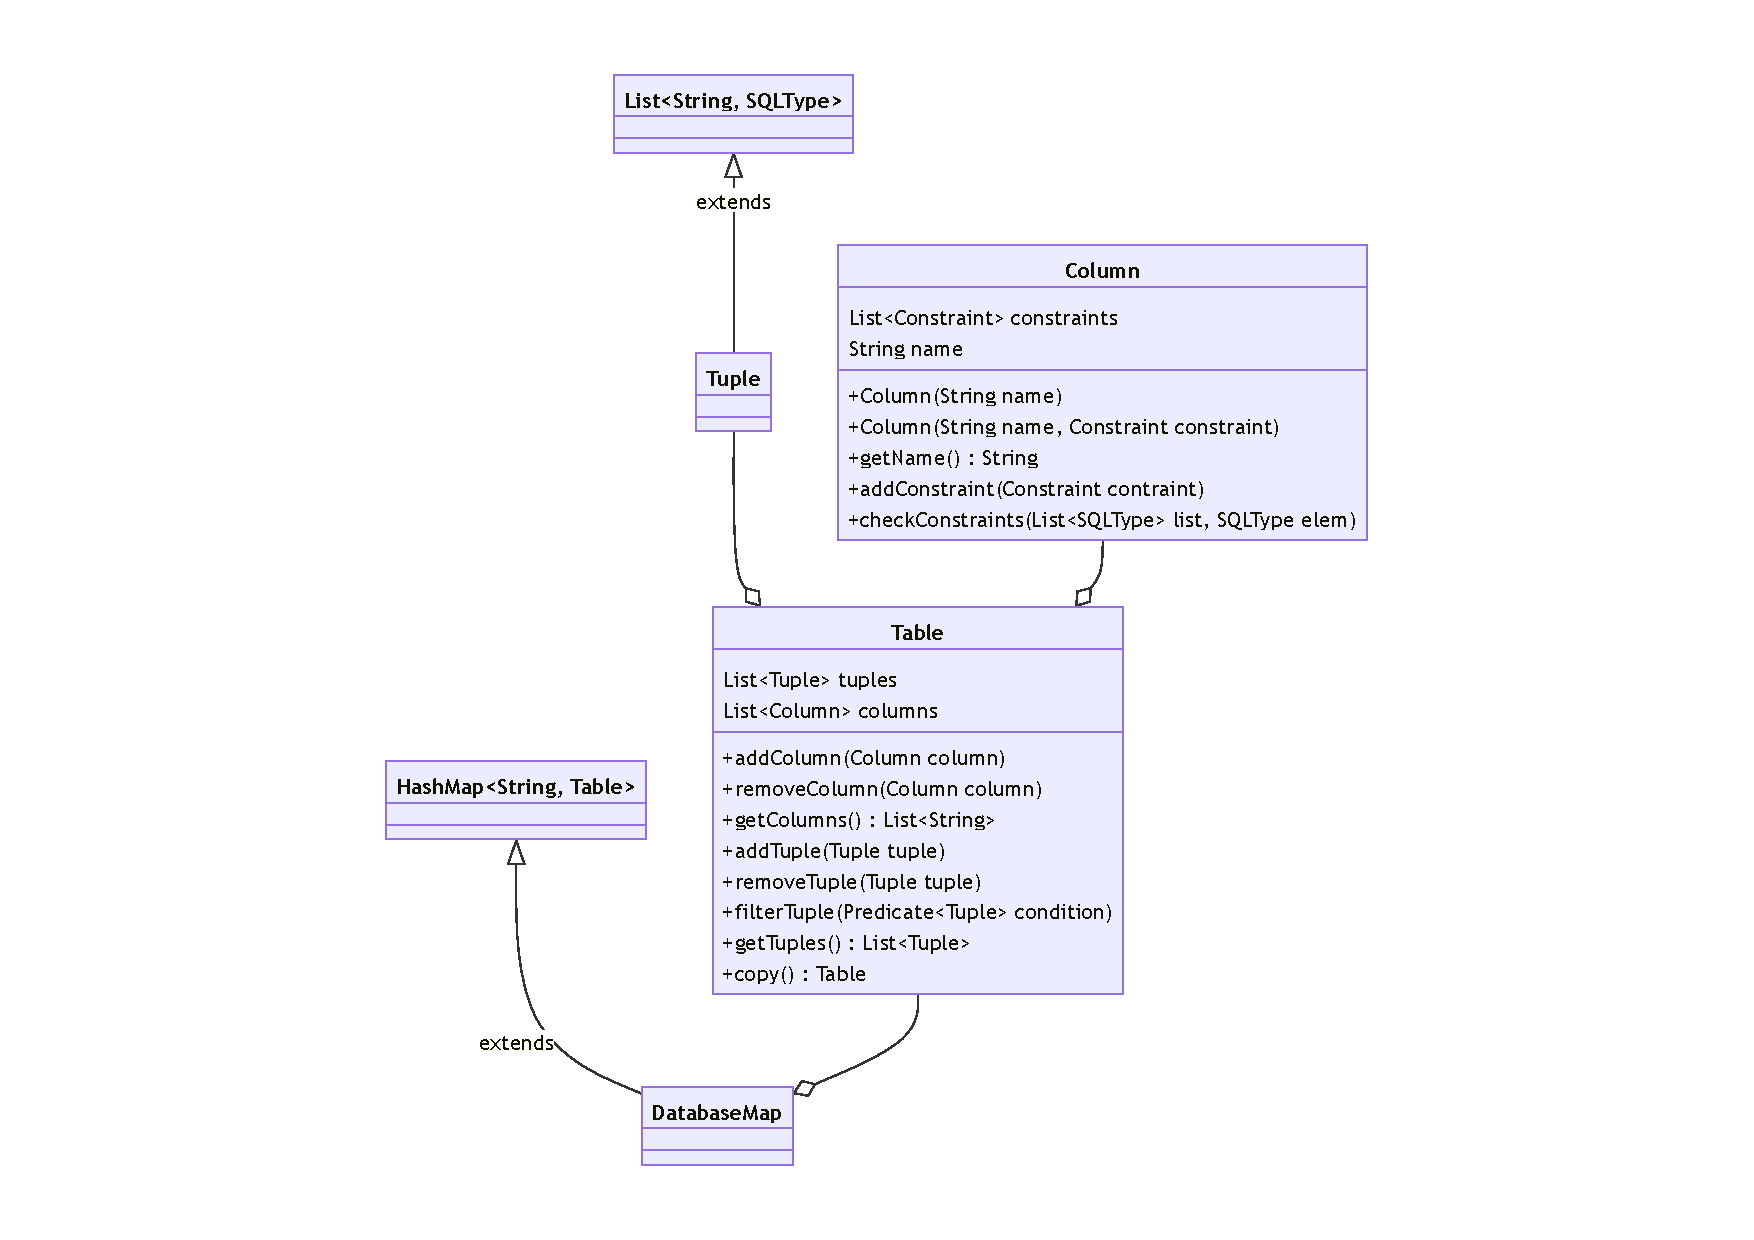
\includegraphics[width=.6\linewidth]{figures/model-diagram.pdf}
    \caption{Schema UML dell'analisi del problema, al suo interno sono rappresentate le entità principali coinvolte nella memorizzazione 
            dei dati e le relazioni tra di esse.}
    \label{fig:model-diagram}
\end{figure}

%----------------------------------------------------------------------------------------
\chapter{Design e Implementazione}
\label{chap:Imple}
%----------------------------------------------------------------------------------------

\section{Architettura}
Ad alto livello, l’architettura del progetto proposto è rappresentata nella \cref{fig:architecture}. Essa si suddivide in due sezioni 
principali, ciascuna delle quali ricopre un ruolo fondamentale per l’implementazione del \ac{DSL}:

\begin{itemize}
\item Parte implementata in Neverlang: Questa sezione si occupa della definizione delle regole sintattiche di \ac{SQL}, descrivendo come 
i vari simboli che compongono la grammatica del \ac{DSL} sono utilizzati e combinati, nonché prodotti. Oltre alla sintassi, Neverlang è 
utilizzato per specificare la semantica del linguaggio, ovvero il comportamento di ciascun costrutto \ac{SQL} durante l’esecuzione. Ogni 
elemento di Neverlang-SQL (ad esempio, \texttt{CREATE TABLE}, \texttt{SELECT}, \texttt{WHERE}, ecc.) è rappresentato utilizzando un modulo Neverlang dedicato, 
all’interno del quale sono definite sia la grammatica che le azioni semantiche necessarie per la corretta interpretazione ed esecuzione 
delle funzioni ad esso associate.
\item Parte implementata in Java: Le classi implementate in questa sezione del progetto sono progettate principalmente per gestire i 
dati memorizzati nelle strutture create appositamente per il dominio sul quale opera \ac{SQL}. Queste classi modellano entità come il 
database, le tabelle, le colonne, le tuple, e i tipi di dati, fornendo metodi per manipolare ciascuna di esse in modo conforme alle 
specifiche del linguaggio.
\end{itemize}

\begin{figure}
\centering
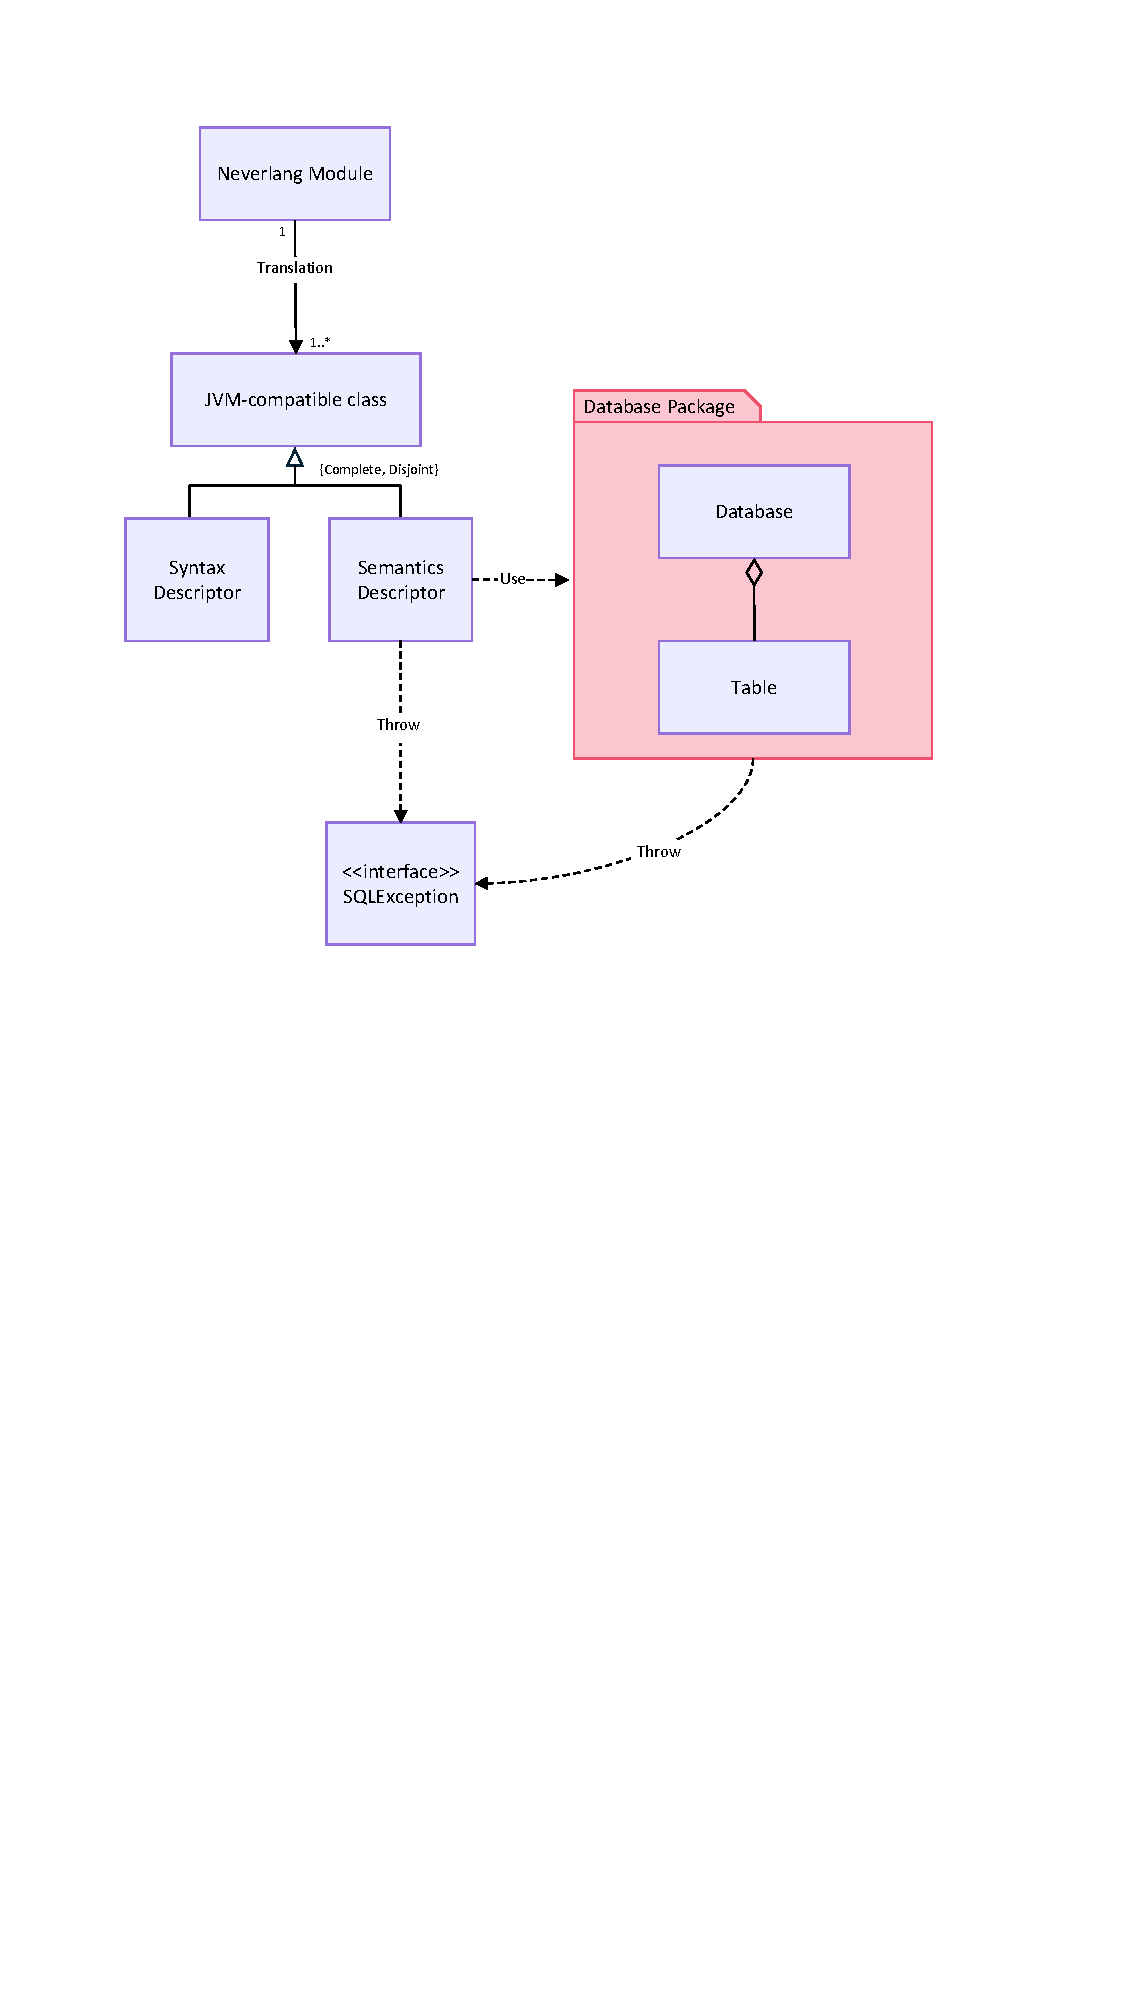
\includegraphics[width=.8\linewidth]{figures/architecture.pdf}
\caption{Diagramma dell’architettura del progetto, illustra le principali dipendenze tra i componenti e i vari moduli.}
\label{fig:architecture}
\end{figure}

Come mostrato nel diagramma in \cref{fig:architecture}, ogni modulo di Neverlang (e le relative specifiche sintattiche e semantiche) 
viene tradotto in file sorgenti compatibili con la \ac{JVM} tramite il compilatore del framework, chiamato \textit{nlgc}. I file così 
generati sono successivamente utilizzati da \textit{javac}\footnote{Javac rappresenta il compilatore principale utilizzato dal 
linguaggio di programmazione Java; si occupa di tradurre il codice sorgente in un formato eseguibile dalla JVM.} per produrre file 
di classe, impiegati per rappresentare gli oggetti Java \cite[p. 19]{Vacchi2015}. In particolare, il codice generato si suddivide 
principalmente in due categorie: sintattiche e semantiche. Infatti, per ogni modulo con annessa una specifica semantica, Neverlang 
produce una classe chiamata convenzionalmente \texttt{<module-name>\$role\$syntax}. Allo stesso modo, per ogni ruolo indicato e per 
ogni non terminale definito all'interno del modulo, viene prodotta una classe atta a descriverne il comportamento, denominata 
\texttt{<module-name>\$role\$<role-name>\$<node-number>} \cite[pp. 21-22]{Vacchi2015}. Le classi di sintassi sono utilizzate per 
verificare che le regole grammaticali siano rispettate nelle query \ac{SQL} fornite in input. Questo processo di validazione si 
propone di controllare che la struttura delle query segua correttamente le specifiche di \ac{SQL}, prevenendo errori comuni di 
sintassi. Di maggiore rilevanza per l’esecuzione del linguaggio è la parte riguardante il comportamento di ogni elemento, gestita 
attraverso le classi di semantica. Ciascuna di queste classi è responsabile di una fase specifica dell’elaborazione ed esecuzione del 
nodo dell’\ac{AST} al quale sono riferite. Queste classi contengono la logica che determina il comportamento esatto di Neverlang-SQL 
durante l’esecuzione delle query, permettendo inoltre di interagire con la parte modellata in Java e che modella il dominio 
all'interno del quale il DSL viene applicato.

Le classi implementate tramite il linguaggio di programmazione Java, come \texttt{Database}, \texttt{Table}, \texttt{Column}, e \texttt{Tuple}, sono strettamente 
integrate con le classi semantiche generate dal compilatore di Neverlang. Questa integrazione permette alle ultime di eseguire 
operazioni dirette sul dominio modellato, quali la modifica della struttura delle tabelle, l’inserimento e la manipolazione dei dati, 
e l’esecuzione di query complesse per ottenere informazioni specifiche richieste dall’utente.

Inoltre, sia le classi Java che quelle generate da Neverlang sono progettate per gestire le eccezioni. Il design proposto in questa 
sezione dell'elaborato include la generazione e la gestione di eccezioni personalizzate, ognuna delle quali rappresenta un errore 
specifico che può verificarsi durante l’analisi o l’esecuzione delle query, come errori di sintassi, accessi non validi ai dati 
od operazioni non consentite.


\section{Sintassi}
La progettazione della sintassi di Neverlang-SQL si basa su una struttura definita suddividendo il linguaggio in cinque macro-aree 
principali: i fondamenti del linguaggio, la gestione delle tabelle, la gestione dei dati, la gestione delle interrogazioni al 
database e l'aggregazione di dati. Ciascuna delle sezioni elencate è definita per soddisfare precisi requisiti del linguaggio ed 
è implementata incrementalmente, in modo da ottenere una versione funzionante del DSL che viene migliorata con ogni aggiunta.

\subsection{Fondamenti del linguaggio}
\label{subsec:fondamenti-linguaggio}
Il design del linguaggio è fondato sull’interpretazione di ogni query ricevuta in input come una sequenza di operazioni 
indipendenti l’una dall’altra, le quali possono essere eseguite in modo sequenziale. Questa struttura sintattica modulare consente 
di ottenere una grande flessibilità nell’esecuzione di operazioni complesse e nella combinazione di più comandi SQL in un’unica 
istruzione. All'interno di questa rappresentazione, il ruolo fondamentale è ricoperto dal simbolo non terminale \texttt{Operation}, 
il quale rappresenta una singola operazione da eseguire, come la creazione di una tabella o l’inserimento di dati.

\paragraph{Unione di più operazioni}
Per supportare la concatenazione di più operazioni in una singola query, viene utilizzato il non terminale \texttt{OperationList}. 
Questo simbolo può rappresentare una singola operazione o una sequenza di operazioni, ognuna delle quali è separata dall’operatore 
punto e virgola (\texttt{;}). Inoltre, \texttt{OperationList} è anche l'elemento utilizzato per definire l'assioma\footnote{Definito 
anche ``simbolo di partenza'', convenzionalmente rappresenta il punto di partenza di ogni linguaggio definito utilizzando Neverlang.} 
del linguaggio: \texttt{Program}.

La definizione ricorsiva della lista, illustrata in \cref{fig:list-ast}, permette di definire sequenze di operazioni di lunghezza 
arbitraria, offrendo agli utenti una discreta flessibilità per la scrittura delle query. Tale struttura non solo facilita 
l’esecuzione di operazioni multiple ma agevola anche l'estensione delle regole grammaticali del DSL: nuovi tipi di operazioni 
potranno essere aggiunti a quelle già esistenti senza dover modificare la sintassi di base proposta nel paragrafo corrente. 
Concludendo, l'approccio modulare proposto non solo migliora la chiarezza del codice ma aumenta anche la manutenibilità del 
linguaggio, permettendo l’aggiornamento o la modifica di singole operazioni senza influire sull’intero sistema.

\begin{figure}[H]
    \centering
    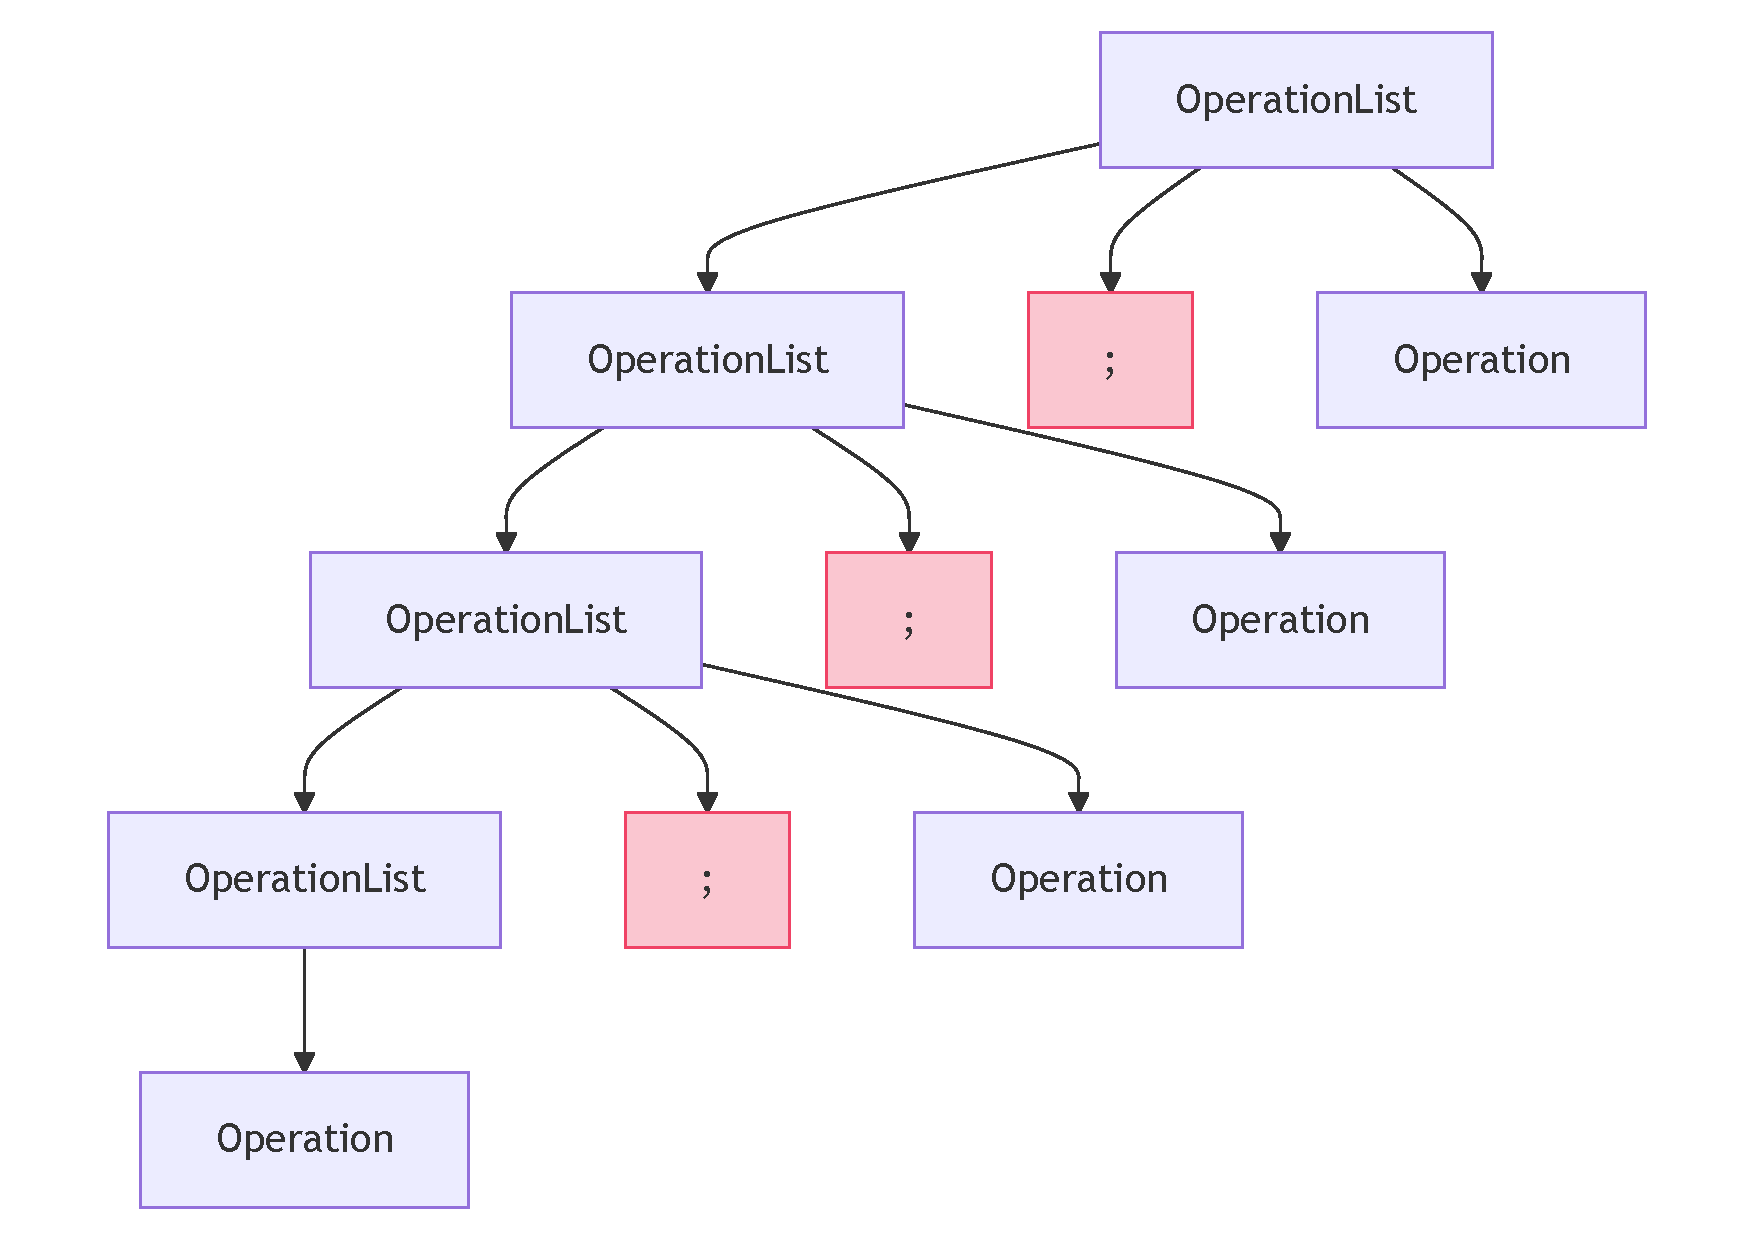
\includegraphics[width=.8\linewidth]{figures/list-ast.pdf}
    \caption{Esempio di albero sintattico di una lista di operazioni}
    \label{fig:list-ast}
\end{figure}

Di seguito viene riportata la definizione della grammatica discussa, illustrando come i vari simboli sono definiti:
\lstinputlisting[
    label={lst:main-grammar},
    language=BNF
]{listings/main-grammar.bnf}
Per poter modellare una grammatica maggiormente flessibile, è stato introdotto anche il simbolo \texttt{EmptyOperation}. La scelta 
è finalizzata a evitare una struttura grammaticale rigida, permettendo così all’utente finale di decidere se concludere l’ultima 
operazione della query con il simbolo terminale (rappresentato dal punto e virgola) oppure no, senza che l’esecuzione generi un 
errore.

\paragraph{Identificare gli elementi}
Un altro componente fondamentale del linguaggio è il simbolo \texttt{Id}, che rappresenta un identificatore univoco per gli 
elementi del database, come tabelle e colonne. \texttt{Id} è modellato tramite un’espressione regolare (\textit{regex}) che consente 
di incapsulare stringhe composte da almeno un carattere alfabetico, seguito opzionalmente da ulteriori caratteri, numeri o un 
carattere di sottolineatura. Questa flessibilità permette a \texttt{Id} di adattarsi a un ampio insieme di convenzioni di 
denominazione, garantendo che gli identificatori siano sempre validi all’interno del contesto del database. L’utilizzo di una 
\textit{regex} permette di validare gli identificatori in modo efficiente durante l’esecuzione, tramite l’uso di pattern o parole 
chiave, riducendo il rischio di errori dovuti a nomi non validi e migliorando così la robustezza del linguaggio\footnote{Uno 
specifico componente di Neverlang, chiamato DEXTER, include al suo interno un analizzatore lessicale che permette di identificare 
i lessemi a tempo d’esecuzione \cite{Dexter2012, Vacchi2015}.}.


\subsection{Gestione delle tabelle}
Le operazioni necessarie per gestire efficacemente le tabelle all’interno del linguaggio Neverlang-SQL sono: \texttt{CREATE TABLE}, \texttt{ALTER 
TABLE} e \texttt{DROP TABLE}. Queste operazioni forniscono agli utenti la capacità di definire nuove tabelle, modificare quelle esistenti o 
rimuoverle dal database. La sintassi delle operazioni descritte è la seguente:
\lstinputlisting[
label={lst:table-grammar},
language=BNF
]{listings/table-grammar.bnf}

Ogni operazione rispetta il principio della modularità discusso nella \cref{subsec:fondamenti-linguaggio}, producendo un elemento 
\texttt{Operation} che rappresenta un’azione completa e indipendente all’interno del DSL. Questa indipendenza permette alle 
operazioni di essere utilizzate singolarmente o concatenate con altre operazioni, offrendo flessibilità nella realizzazione delle 
query.\\\\
Considerando che \texttt{CREATE TABLE} è il costrutto con la sintassi più complessa tra quelli definiti, esso viene utilizzato come esempio 
per illustrare il funzionamento di queste operazioni.

\begin{figure}
\centering
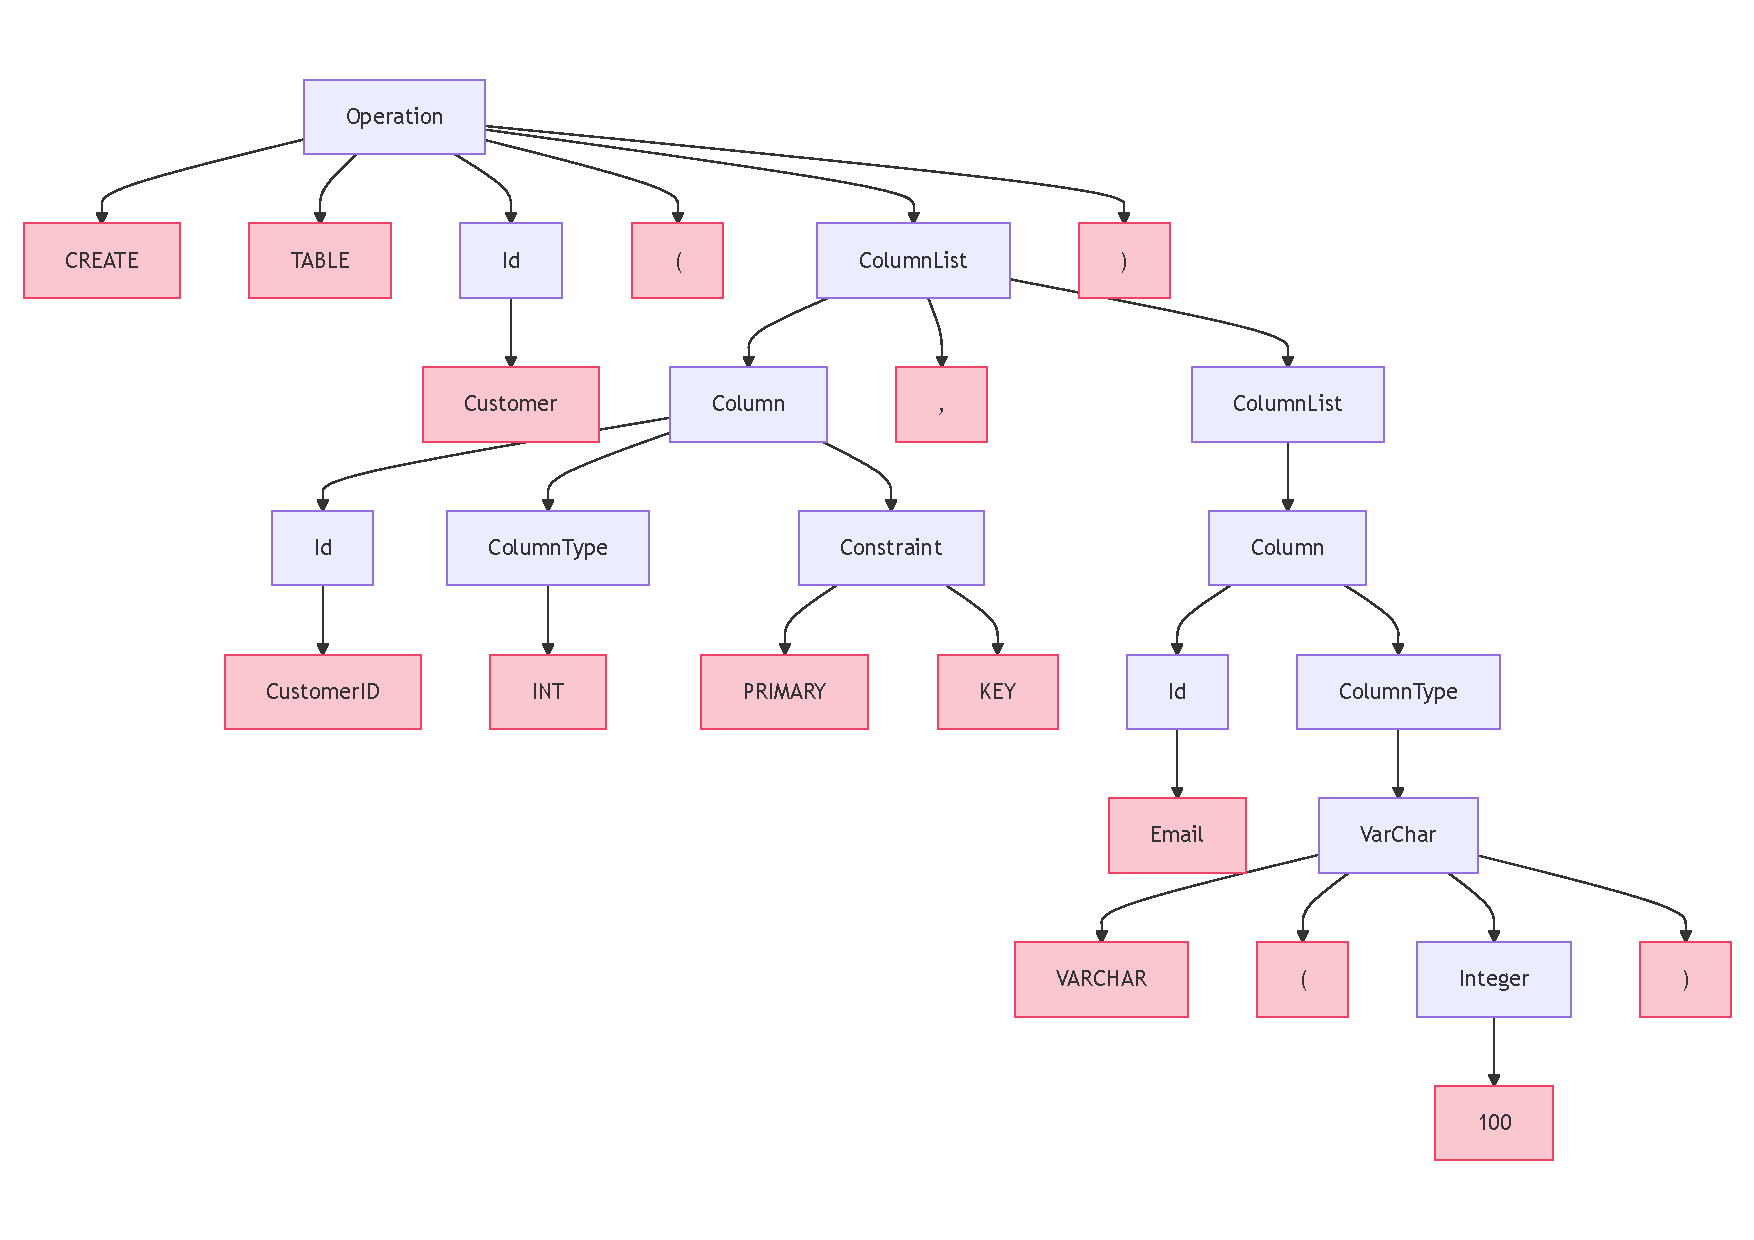
\includegraphics[width=.9\linewidth]{figures/create-table-ast.pdf}
\caption{Illustrazione rappresentante un esempio di albero sintattico generato per la creazione di una tabella.}
\label{fig:create-table-ast}
\end{figure}

Nella \cref{fig:create-table-ast} viene presentato un AST generato dall’esecuzione di una query, la quale ha come obiettivo la 
creazione di una nuova tabella all’interno del database. In rosso sono indicati i simboli terminali, mentre in blu sono indicati i 
simboli non terminali. La struttura dell’albero riflette la gerarchia e le dipendenze tra i diversi componenti della query, 
mostrando come ciascun elemento della sintassi viene interpretato dal linguaggio. In particolare, l’operazione d’esempio richiede 
la creazione di una tabella chiamata Customer, contenente due attributi. Il primo attributo, definito come chiave primaria (che non 
può essere nullo e deve essere unico per ogni tupla inserita nella tabella), rappresenta il numero intero identificativo di ogni 
cliente ed è chiamato ``CustomerID''. Questo attributo è progettato per garantire l’unicità di ogni cliente all’interno del database, 
essendo un elemento essenziale per mantenere l’integrità dei dati. Il secondo attributo previsto per la tabella Customer è la 
colonna ``Email'', che è destinata a contenere l’indirizzo email di ogni cliente. Questa colonna è definita come una stringa con una 
lunghezza massima di 100 caratteri, garantendo così che tutti gli indirizzi email inseriti rispettino un formato standardizzato e 
un limite di lunghezza specificato.

All’interno dell’albero proposto possiamo individuare anche altri importanti elementi utilizzati per definire in modo chiaro la 
tabella da inserire:
\begin{itemize}
    \item \textbf{Tipologie di dati}: Sono definiti i tipi di dati supportati per le colonne della tabella ed includono \texttt{INT}, 
    \texttt{FLOAT}, \texttt{VARCHAR} e \texttt{BOOLEAN}. Questi tipi di dati rappresentano le principali opzioni per quanto concerne 
    la gestione delle informazioni all’interno di un database, consentendo la rappresentazione di numeri interi, numeri decimali, 
    stringhe di testo e valori booleani. In particolare, la definizione della stringa prevede anche la precisazione del numero 
    massimo di caratteri accettati\footnote{Il numero massimo di caratteri di \texttt{VARCHAR} rappresenta un particolare esempio 
    di vincolo implicito sui dati da inserire nella colonna. Un altro esempio è che il tipo del dato deve corrispondere al tipo 
    specificato nella dichiarazione della colonna.}.
    \item \textbf{Vincoli}: Quando si definisce una tabella, e in particolare i suoi attributi, possono essere esplicitati una serie 
    di vincoli che devono essere rispettati dai dati per garantirne l’integrità. I vincoli supportati includono \texttt{UNIQUE}, 
    che garantisce l’unicità dei valori in una colonna, \texttt{NOT NULL}, che assicura che una colonna non contenga valori nulli, 
    e \texttt{PRIMARY KEY}, che identifica univocamente ogni riga all’interno della tabella e non permette valori duplicati.
\end{itemize}

\subsection{Gestione dei dati}
La gestione dei dati in Neverlang-SQL include le operazioni fondamentali per manipolare i dati all’interno delle tabelle del database. 
Le principali operazioni supportate in questa macro-area sono \texttt{INSERT}, \texttt{UPDATE} e \texttt{DELETE}. Rispettivamente, queste 
operazioni permettono agli utenti di aggiungere nuove righe, modificare i dati esistenti e rimuovere righe dalle tabelle. La 
sintassi di queste operazioni è:
\lstinputlisting[
    label={lst:data-grammar},
    language=BNF
]{listings/data-grammar.bnf}

Ogni operazione è progettata per essere intuitiva e riflettere le operazioni comunemente utilizzate nei sistemi SQL. L’operazione 
\texttt{INSERT} permette di specificare una lista di colonne in cui inserire i valori e una lista di valori corrispondenti. L’operazione 
\texttt{UPDATE} consente di modificare i valori esistenti in una o più colonne specificando una condizione per filtrare le righe da 
aggiornare. Infine, l’operazione \texttt{DELETE} permette di rimuovere un sottoinsieme di righe da una tabella.

L’inclusione di queste operazioni all’interno di Neverlang-SQL consente agli utenti di gestire i dati in modo flessibile e robusto, 
garantendo al contempo che tutte le modifiche ai dati siano conformi alle regole di integrità definite all’interno del database. 
Ogni operazione di gestione dei dati è progettata per essere un’operazione \texttt{Operation} indipendente, che può essere 
utilizzata singolarmente o combinata con altre operazioni in una singola query.

\paragraph{Liste di oggetti}
Le liste \texttt{IdList}, \texttt{ValueList} e \texttt{SetList} sono progettate in modo analogo alla lista di operazioni 
\texttt{OperationList} descritta nella \cref{subsec:fondamenti-linguaggio}. Questa progettazione consente di rappresentare sequenze 
flessibili di identificatori, valori e assegnazioni nelle query SQL, permettendo di specificare un numero variabile di elementi 
secondo le necessità dell’utente. Ogni lista può contenere uno o più elementi, utilizzando una struttura ricorsiva che facilita la 
costruzione di query articolate e complesse.

\paragraph{Tipi di valori}
I valori utilizzati nelle query sono definiti in base a un insieme di tipologie predefinite, ciascuna caratterizzata da un formato 
specifico che il linguaggio è in grado di riconoscere. I tipi di valori supportati in Neverlang-SQL includono:
\begin{itemize}
    \item \textbf{Stringhe}: Le stringhe sono rappresentate come sequenze di caratteri racchiuse tra virgolette singole o doppie. 
    Neverlang-SQL riconosce le stringhe che possono includere caratteri speciali, garantendo che l’intero contenuto tra le virgolette 
    sia trattato come un unico valore di testo.
	\item \textbf{Interi}: I valori interi sono numeri composti da una sequenza di cifre, che possono essere preceduti da un segno 
    positivo o negativo. All'interno del progetto, sono considerati validi i valori che rappresentano quantità discrete, formati 
    correttamente come numeri interi e senza parti decimali.
	\item \textbf{Numeri in virgola mobile}: Questi valori rappresentano numeri con una parte decimale. Possono includere un segno 
    positivo o negativo e supportano anche la notazione scientifica con un esponente (ad esempio ``1.23e-2'' rappresenta il numero 
    $1.23 \times 10^{-2}$, ossia $0.0123$ ). Questo consente di rappresentare una vasta gamma di valori numerici, inclusi numeri 
    molto piccoli o molto grandi con precisione.
	\item \textbf{Booleani}: I valori booleani sono rappresentati dalle parole chiave \texttt{TRUE} o \texttt{FALSE}. Questi valori 
    sono utilizzati per indicare stati di verità binari e vengono riconosciuti come tali solo quando corrispondono esattamente a 
    una delle due parole chiave, garantendo un’interpretazione corretta nelle operazioni logiche.
	\item \textbf{Valori Nulli}: Il valore \texttt{NULL} indica l’assenza di un valore. È una parola chiave specifica che 
    Neverlang-SQL riconosce per rappresentare la mancanza di dati in un campo. Questo valore è trattato in modo distinto dagli 
    altri tipi, permettendo di gestire dati mancanti o opzionali all’interno del database.
\end{itemize}

\paragraph{Espressioni booleane}
Il linguaggio sviluppato supporta tre tipologie principali di funzioni booleane, ognuna progettata per offrire flessibilità e 
potenza espressiva nella costruzione di query complesse. Queste funzioni sono fondamentali per il filtraggio e l’estrazione dei dati 
dal database, consentendo agli utenti di definire criteri di selezione precisi e ottimizzati.
\begin{itemize}
    \item La prima tipologia di funzioni booleane riguarda i confronti diretti tra attributi di una colonna e un valore specificato 
    dall’utente. Queste funzioni permettono di eseguire confronti utilizzando operatori come \texttt{=}, \texttt{<>}, \texttt{<}, \texttt{>}, \texttt{<=}, e \texttt{>=}. Ad esempio, è 
    possibile selezionare tutte le righe di una tabella in cui il valore di una colonna specifica è maggiore di un certo numero, o 
    dove un campo di testo corrisponde esattamente a una stringa specificata. Questa capacità di confronto diretto è essenziale per 
    operazioni di filtraggio di base, fornendo un controllo sui dati che vengono recuperati dal database.

    \item La seconda tipologia si concentra sulle funzioni booleane native di SQL, come \texttt{BETWEEN}, \texttt{IN} e \texttt{IS NULL}. Queste funzioni sono 
    particolarmente utili per eseguire controlli più complessi e specifici. Ad esempio, la funzione \texttt{BETWEEN} permette di verificare 
    se un valore rientra all’interno di un determinato intervallo, mentre \texttt{IN} consente di verificare se un valore appartiene a un 
    insieme predefinito di valori. Queste funzioni forniscono un modo semplice e intuitivo per esprimere condizioni che coinvolgono 
    intervalli o insiemi, rendendo le query più leggibili e facili da scrivere. Infine, la funzione \texttt{IS NULL} è utilizzata per 
    ricercare tuple con precisi attributi non dichiarati.

    \item La terza tipologia è rappresentata dalla capacità di combinare espressioni booleane pre-esistenti tramite operatori logici 
    come \texttt{AND}, \texttt{OR} e \texttt{NOT}. Questa funzionalità consente agli utenti di creare condizioni più complesse ed articolate, combinando più 
    criteri di selezione in una singola operazione. Ad esempio, è possibile costruire una query che seleziona tutte le righe in cui 
    un attributo è maggiore di un certo valore e un altro attributo corrisponde a una stringa specifica, oppure che recupera tutte 
    le righe in cui un attributo non è uguale a un determinato valore o rientra in un intervallo specificato. L’uso di \texttt{NOT} permette 
    di escludere determinati risultati, invertendo la logica delle condizioni definite.
\end{itemize}
Queste operazioni sono particolarmente utili per la gestione della selezione dei dati da aggiornare nelle operazioni \texttt{UPDATE}, in cui 
la precisione nella definizione dei criteri di modifica è fondamentale per garantire la modifica richiesta dall'utente finale. 
Inoltre, le stesse funzioni booleane saranno utilizzate dagli operatori di selezione, di cui si parlerà nella 
\cref{subsec:interrogazioni}, per selezionare le informazioni che l'utente vuole ottenere dal database.

\subsection{Interrogazioni al database}
\label{subsec:interrogazioni}
Le interrogazioni al database rappresentano una delle funzionalità essenziali di Neverlang-SQL, consentendo agli utenti di estrarre, 
filtrare e ordinare dati in base a criteri specifici. Le operazioni di interrogazione implementate nel linguaggio includono \texttt{SELECT}, 
\texttt{FROM}, \texttt{WHERE} e \texttt{ORDER BY}. Queste operazioni permettono di recuperare informazioni strutturate dalle tabelle, applicare filtri per 
ottenere solo i dati rilevanti e ordinare i risultati secondo criteri definiti dall’utente. La combinazione di queste operazioni 
permette di costruire query complesse e dettagliate, rispondendo a diverse esigenze di analisi dei dati.

La grammatica per le operazioni di interrogazione in Neverlang-SQL è progettata in modo da fornire una struttura flessibile e 
modulare. Le regole grammaticali per le interrogazioni sono le seguenti:
\lstinputlisting[
label={lst:data-op-grammar},
language=BNF
]{listings/data-op-grammar.bnf}

Questa definizione grammaticale consente di costruire query che selezionano, filtrano e ordinano i dati in modo estremamente 
flessibile. Un elemento chiave di questa progettazione è l’uso del simbolo \texttt{SelectedData} sia come input che come output per 
le diverse operazioni. Questo approccio garantisce la coerenza nella sintassi delle query e permette di combinare le operazioni in 
modo fluido, senza restrizioni rigide sulla loro sequenza. La scelta di strutturare le operazioni in modo che ogni operazione di 
interrogazione utilizzi e restituisca il simbolo \texttt{SelectedData} è fondamentale per mantenere la flessibilità del linguaggio. 
Tramite questa configurazione, l’output di una clausola come \texttt{WHERE} può essere utilizzato direttamente come input per un’altra 
operazione, come \texttt{ORDER BY} o \texttt{SELECT}. Questo significa che le operazioni possono essere combinate in modo flessibile, senza che una 
dipenda necessariamente dall’altra. Ad esempio, una query potrebbe iniziare con la selezione di tutte le colonne da una tabella 
(\texttt{SELECT}), seguita da un filtro sui dati recuperati (\texttt{WHERE}) e, infine, ordinare i risultati secondo una 
specifica colonna (\texttt{ORDER BY}). In alternativa, potrebbe omettere l’operazione \texttt{WHERE} e includere solo \texttt{ORDER BY}. Grazie all’uso 
ricorsivo di \texttt{SelectedData}, ogni operazione aggiunge una trasformazione sui dati senza la necessità di definire 
esplicitamente tutte le altre operazioni all’interno della grammatica.

Di seguito sono riassunti i principali vantaggi ottenuti dall’utilizzo di tale struttura:
\begin{itemize}
    \item Modularità e coerenza: Utilizzando lo stesso simbolo \texttt{SelectedData} per rappresentare il risultato di qualsiasi 
    operazione di interrogazione, il linguaggio mantiene una coerenza sintattica che semplifica l’apprendimento e l’uso da parte degli 
    utenti. La modularità della grammatica permette di definire operazioni complesse senza introdurre ambiguità o conflitti sintattici.
    \item Estensibilità del linguaggio: La struttura progettuale facilita l’espansione del linguaggio. Poiché ogni nuova operazione di 
    interrogazione può essere definita come una trasformazione che prende in input \texttt{SelectedData} e restituisce un altro 
    \texttt{SelectedData}, è possibile aggiungere nuove operazioni seguendo lo stesso modello senza modificare la struttura di base del 
    linguaggio. Ad esempio, l’aggiunta della clausola \texttt{GROUP BY}, che verrà approfondita nella \cref{sec:aggregazione}.
    \item Flessibilità nella costruzione delle query: Gli utenti possono combinare liberamente le operazioni di interrogazione, 
    utilizzandone un sottoinsieme a scelta, senza essere vincolati da una sequenza rigida di operazioni. Questo rende il linguaggio 
    particolarmente adatto per scenari complessi di analisi dei dati, dove le esigenze di interrogazione possono variare notevolmente.
    \item Facilità di manutenzione ed evoluzione: Grazie alla sua struttura modulare, il linguaggio è facile da mantenere e 
aggiornare. Nuove funzionalità possono essere aggiunte senza richiedere significative riscritture del codice esistente. Questo 
rende Neverlang-SQL non solo robusto ma anche sostenibile nel lungo termine.
\end{itemize}

L’approccio alle operazioni di interrogazione proposto, basato sull’uso ricorsivo e flessibile del simbolo \texttt{SelectedData}, 
offre un equilibrio ideale tra potenza espressiva e semplicità sintattica. Questo design non solo rende il linguaggio facile da 
imparare e utilizzare, ma ne facilita anche l’espansione futura per supportare nuove funzionalità e requisiti di interrogazione 
avanzati. La capacità di combinare operazioni senza restrizioni rigide rende il linguaggio considerevolmente più versatile per 
l’interrogazione del database.

\subsection{Aggregazione di dati}
\label{sec:aggregazione}
L’aggregazione di dati è una funzionalità avanzata di Neverlang-SQL che permette di raggruppare i dati e calcolare valori aggregati 
come conteggi, somme, medie, minimi e massimi. Queste operazioni sono essenziali per l’analisi dei dati, consentendo agli utenti di 
ottenere informazioni riassuntive da collezioni di dati di grandi dimensioni e di esplorare pattern e tendenze al loro interno.

Per supportare l’aggregazione di dati, è necessario adattare la clausola \texttt{SELECT} in modo che sia compatibile con i requisiti imposti 
dalla clausola \texttt{GROUP BY}. Questa scelta è dovuta al fatto che, quando i due operatori sono utilizzati in combinazione, gli 
\texttt{Id} specificati dalla \texttt{SELECT} non rappresentano più solamente gli attributi da estrarre ma anche quelli da generare tramite 
l’aggregazione. Per questo motivo, la grammatica è definita come segue:
\lstinputlisting[
label={lst:aggregate-grammar},
language=BNF
]{listings/aggregate-grammar.bnf}

Per operare correttamente, è necessario un controllo rigoroso tra gli identificatori (\texttt{Id}) elencati nella clausola 
\texttt{SELECT} e quelli presenti nella clausola \texttt{GROUP BY}. In SQL standard, tutti gli identificatori specificati nella 
clausola \texttt{SELECT} devono essere o inclusi nella clausola \texttt{GROUP BY} o essere utilizzati all’interno di una funzione 
di aggregazione (come \texttt{SUM}, \texttt{AVG}, \texttt{MAX}, \texttt{MIN}, \texttt{COUNT}). Questo vincolo garantisce che le 
query restituiscano risultati significativi e coerenti, poiché solo i dati che sono stati raggruppati possono essere utilizzati 
per calcolare valori aggregati\footnote{Il vincolo descritto è fondamentale e l’obiettivo dell’implementazione semantica del 
costrutto è la sua corretta individuazione}.

Le funzioni di aggregazione sono trattate come elementi identificativi (\texttt{Id}) all’interno della grammatica del progetto, il 
che consente di utilizzarle in modo flessibile all’interno delle query. La grammatica per le funzioni di aggregazione è definita 
come segue:
\lstinputlisting[
label={lst:aggregate-fun-grammar},
language=BNF
]{listings/aggregate-fun-grammar.bnf}

Queste definizioni mostrano come le funzioni di aggregazione siano modellate. In particolare, la funzione \texttt{COUNT} può essere 
applicata a un attributo o all’intera tabella usando l’asterisco (\texttt{*}), per contare tutte le righe che soddisfano i criteri 
della query. Le altre funzioni di aggregazione, come \texttt{SUM}, \texttt{AVG}, \texttt{MAX} e \texttt{MIN}, sono applicate 
specificamente a una colonna, calcolando rispettivamente la somma, la media, il valore massimo e il valore minimo dei dati 
raggruppati.

Modellando le funzioni di aggregazione come identificatori, Neverlang-SQL consente di integrarli direttamente nelle query come 
parte degli identificatori nella clausola \texttt{SELECT}. Questo approccio semplifica la sintassi e mantiene la coerenza del 
linguaggio, consentendo agli utenti di includere funzioni di aggregazione insieme ad altri identificatori nella stessa lista di 
selezione.

\section{Semantica}
La semantica del DSL ricopre il ruolo di definire il comportamento operativo che le diverse costruzioni sintattiche del linguaggio dovranno 
rispettare durante l’esecuzione. Mentre la sintassi stabilisce le regole su come devono essere strutturate le query per essere considerate 
valide, la semantica si concentra su cosa tali query effettivamente fanno quando vengono eseguite. In particolare, l’implementazione della 
sintassi è realizzata utilizzando il linguaggio di programmazione Java e le sue librerie, nonché le classi modellate ad-hoc per il dominio 
applicativo del progetto\footnote{Questo comportamento è necessario perché Neverlang include solo una piccola libreria di funzioni di 
utilità. In generale, viene incoraggiato l’utilizzo delle librerie standard appartenenti all’ecosistema Java \cite{Vacchi2015}.}.

All’interno del capitolo corrente sono esplorate le diverse fasi del processo semantico, che comprendono il controllo della struttura, la 
valutazione e la gestione dell’output.

\subsection{Fase di controllo della struttura}
A causa dell’alto grado di libertà concesso dalla sintassi delle operazioni utilizzate nelle interrogazioni del database\footnote{Il 
riferimento è alla scelta implementativa delle operazioni utilizzate nell’interrogazione del database, che utilizzano, sia come input che 
come output, un elemento \texttt{SelectedData} (\cref{subsec:interrogazioni}).}, Neverlang-SQL include una fase preliminare di 
controllo della struttura. In questa fase, il linguaggio verifica che la struttura complessiva della query sia accettabile e coerente con le 
regole semantiche definite. Ad esempio, non è permesso includere una clausola \texttt{ORDER BY} senza prima specificare una tabella da cui 
selezionare i dati, né è possibile filtrare una tabella tramite l’operazione \texttt{WHERE} senza specificare come utilizzarne l’output, ad 
esempio, tramite \texttt{SELECT} o \texttt{DELETE}.

Il controllo della struttura assicura che le query rispettino una logica operativa sequenziale appropriata, impedendo che vengano eseguite 
operazioni che non abbiano un contesto di riferimento valido o che manchino di informazioni essenziali per l’elaborazione. Questa fase è 
fondamentale per evitare errori comuni e garantire che le query siano costruite in modo da poter essere valutate correttamente nelle fasi 
successive.

\subsection{Fase di valutazione}
La fase di valutazione rappresenta il nucleo del processo semantico di Neverlang-SQL. In questa fase, la maggior parte delle regole 
sintattiche del linguaggio vengono analizzate per determinare l’azione esatta che ciascun elemento della query deve eseguire. Durante la 
valutazione, vengono interpretati i vari componenti della query, come selezioni, filtraggi, ordinamenti e aggregazioni, per determinare come 
interagiscono tra loro e quali operazioni specifiche devono essere eseguite sul database. Questa fase traduce essenzialmente le istruzioni 
della query da una rappresentazione sintattica a un insieme di operazioni concrete che manipolano i dati o le tabelle nel database.

\subsection{Fase di output}
Dopo che tutte le operazioni definite nella fase di valutazione sono state eseguite, si passa alla fase di output. In questa fase, viene 
fornito all’utente il risultato finale della query, se presente. L’output può includere l’elenco dei dati selezionati, i risultati delle 
funzioni di aggregazione o altre informazioni richieste dalla query.

La presentazione dei risultati all’utente è considerata una fase indipendente perché la clausola che specifica l’output da fornire non 
rappresenta necessariamente l’ultima operazione eseguita. Per questo motivo, l’esecuzione delle operazioni di ogni elemento del linguaggio 
avviene prima, e solo successivamente il risultato ottenuto viene fornito. Ad esempio, la clausola \texttt{SELECT} indica l’inizio di una 
query di interrogazione e al tempo stesso precisa quali sono gli attributi da fornire come output, ma potrebbe non rappresentare l’ultima 
operazione da eseguire. In caso fosse presente un’operazione di \texttt{ORDER BY}, infatti, sarebbe quest’ultima l’operazione terminale 
eseguita sui dati.

\section{Tecnologie utilizzate}

\subsection{Gradle}
Gradle\footnote{Documentazione di Gradle: https://docs.gradle.org/current/userguide/userguide.html} è un sistema di automazione della 
compilazione del codice, open source, ampiamente utilizzato per progetti in Java, ma supporta anche linguaggi come Scala e JavaScript, ed è 
lo standard per la programmazione in Kotlin e per lo sviluppo di applicazioni per dispositivi Android. Supporta la gestione delle dipendenze, 
la compilazione del codice, l’esecuzione di test e la creazione di pacchetti eseguibili. È estremamente configurabile ed estendibile, 
consentendo di personalizzare il processo di build in base alle specifiche esigenze del singolo progetto.

All’interno di Neverlang-SQL, l’utilizzo di Gradle ha contribuito ad agevolare il processo di compilazione del codice scritto in Neverlang, a 
velocizzare il testing del linguaggio ottenuto ed ha ricoperto un ruolo fondamentale per la gestione delle dipendenze, in particolare con le 
librerie di Neverlang.

\subsection{JUnit5}
JUnit\footnote{Documentazione di JUnit5: https://junit.org/junit5/docs/current/user-guide/} è uno dei framework di unit testing più diffusi 
per il linguaggio di programmazione Java e fornisce un ambiente di test sistematico e automatizzato che aiuta a verificare la correttezza del 
codice.

In particolare, all’interno del progetto è stato utilizzato JUnit Jupyter per testare se il linguaggio generato con Neverlang funzionasse 
correttamente. Questo approccio ha consentito di risparmiare una notevole quantità di tempo in quanto, tramite dei test significativi, è stato 
possibile comprendere rapidamente se le soluzioni implementate fossero corrette oppure no. L’integrazione di JUnit con Gradle ha permesso di 
eseguire i test in modo continuo e di generare report di test dettagliati, agevolando l’individuazione e la risoluzione dei \textit{bug}.

\subsection{Git}
Git\footnote{Documentazione di Git: https://git-scm.com/doc} è un software per il controllo di versione distribuito. Viene ampiamente 
utilizzato per la sua efficienza e flessibilità e permette a uno o più sviluppatori di lavorare ad un progetto gestendone multiple versioni e 
facilitando la collaborazione con terzi.

Durante lo sviluppo del linguaggio, Git (in particolare tramite la piattaforma GitHub) ha permesso di gestire efficacemente le versioni del 
codice e di tracciare ogni singola modifica apportata al progetto. Git ha dunque permesso di sperimentare nuove funzionalità e di correggere 
i bug generati durante lo sviluppo senza il rischio di compromettere il codice stabile. Inoltre, sfruttando gli strumenti per la gestione dei 
branch, è stato possibile sviluppare e testare nuove funzionalità in un ambiente isolato, per poi integrarle nel progetto principale solamente 
dopo essere state testate.

\subsection{CheckStyle}
CheckStyle\footnote{Documentazione di CheckStyle: https://checkstyle.sourceforge.io} è uno strumento di analisi del codice open source, 
progettato per aiutare gli sviluppatori a scrivere codice Java seguendo le convenzioni di stile. CheckStyle verifica che il codice rispetti 
un insieme di regole predefinite, come quelle riguardanti la formattazione, la nomenclatura, la gestione delle eccezioni, ecc. Utilizzando 
questo strumento, è possibile rilevare automaticamente le violazioni dello stile di codice durante il processo di build, riducendo così la 
probabilità di errori e migliorando la leggibilità del codice.

Nel progetto Neverlang-SQL, CheckStyle è stato utilizzato per garantire che il codice Java (escluso quello generato dal compilatore di 
Neverlang, nlgc) rispettasse le convenzioni di stile standard. Questo ha contribuito a mantenere un codice pulito e leggibile, migliorando 
la qualità del codice prodotto.

\subsection{SpotBugs}
SpotBugs\footnote{Documentazione di SpotBugs: https://spotbugs.readthedocs.io/en/stable/} è uno strumento di analisi del codice per il 
linguaggio Java che rileva bug e vulnerabilità potenziali. SpotBugs si concentra sull’identificazione di possibili errori nel codice, come 
dereferenziazioni di nulli, errori logici, problemi di sicurezza e altre pratiche di programmazione sconsigliate che potrebbero causare 
malfunzionamenti o vulnerabilità del software.

Nel contesto del progetto Neverlang-SQL, SpotBugs è stato utilizzato per esaminare il codice Java associato ai moduli di Neverlang e alle 
classi Java, e per identificare eventuali difetti o punti deboli nel codice del linguaggio. Questo strumento ha permesso di migliorare la 
robustezza e la sicurezza del progetto, identificando rapidamente potenziali problemi prima che potessero causare malfunzionamenti nel 
progetto.

%----------------------------------------------------------------------------------------
\chapter{Validazione e Conclusioni}
\label{chap:conclusioni}
%----------------------------------------------------------------------------------------
\section{Validazione}
\label{chap:validazione}
La validazione del progetto realizzato ha interessato principalmente due tipi di controlli: il test sulla struttura dati creata 
e il test sull’output fornito. L’obiettivo del controllo è stato quello di determinare se l’implementazione realizzata 
corrispondesse a ciò che era ragionevolmente atteso che il software facesse.

\subsection{Test della struttura}
\label{section:test-strutt}
Il controllo della base di dati realizzata è stato eseguito sul database creato durante l’esecuzione, costruito usando il file 
utilizzato come sorgente o lo script fornito al test dall’assioma del linguaggio Neverlang, ossia il simbolo \texttt{Program}. In 
questo modo, nei test implementati nel progetto, è stato sufficiente utilizzare l’attributo \texttt{db} del nodo radice dell’AST 
per verificare che la struttura ottenuta corrispondesse a quella attesa dai comandi oggetto di testing.

Nel \cref{lst:simple-test} viene fornito un esempio introduttivo di come i controlli della struttura del database e delle tabelle 
siano stati realizzati. Il punto fondamentale è quello riportato alla riga 12, che corrisponde all’ottenimento dell’attributo 
contenente il database creato dal codice utilizzato come input. In modo del tutto analogo, all’interno dei test “strutturali” del 
progetto, contenuti nella classe \texttt{TableTests.java}, sono eseguiti dei codici d’esempio per verificare se l’output ottenuto 
è quello desiderato.

\lstinputlisting[
float,
label={lst:simple-test},
language=Java,
numbers=left,
frame=none,
caption={Metodo utilizzato per il test del codice prodotto. In particolare, verifica se il nodo radice restituisce un database e se 
al suo interno contiene la tabella creata.}
]{listings/simple-test.txt}

Per poter eseguire i test descritti, è stato fondamentale l’utilizzo della libreria di Neverlang progettata per interagire con 
JUnit\footnote{Repository dell’estensione neverlang-junit: \href{https://maven.adapt-lab.di.unimi.it/\#/neverlang/releases/it/unimi/di/adaptlab/neverlang-junit-extension}{https://maven.adapt-lab.di.unimi.it}}, 
che è stata aggiunta come dipendenza del progetto tramite Gradle. Grazie all’utilizzo di questa estensione e delle annotazioni 
\texttt{@ExtendWith}, \texttt{@NeverlangUnit} e \texttt{@NeverlangUnitParam} definite al suo interno, è stato possibile effettuare 
i test generando in modo automatizzato l’albero sintattico prodotto da Neverlang.

\subsection{Test dell’output fornito}
Il controllo dell’output fornito è stato più complesso, poiché le operazioni di output non modificano la struttura effettiva del 
database, ma ne creano una temporanea utilizzata per generare l’output secondo le richieste dell’utente. Prendendo come esempio la 
query di selezione \texttt{SELECT Nome, Cognome FROM Customers} e assumendo che la tabella sorgente contenga più attributi 
rispetto ai due richiesti, il controllo della struttura della tabella non sarebbe sufficiente, in quanto includerebbe anche altri 
attributi non pertinenti.

\paragraph{Prima implementazione}
Per risolvere il problema descritto, inizialmente è stato aggiunto nel progetto un attributo al nodo radice chiamato “output”, 
utilizzato per salvare la tabella temporanea generata dalla query di input, con un funzionamento simile a quello descritto nella 
\cref{section:test-strutt} riguardo al test della struttura della tabella. Tuttavia, questo approccio si è rivelato poco flessibile, 
poiché richiedeva di mantenere un secondo database fittizio, che poteva generare errori se l’utente avesse voluto creare un database 
con lo stesso nome. Inoltre, obbligava la parte semantica a gestire un aspetto non richiesto dal progetto e introduceva delle 
problematiche riguardo alla memorizzazione dell’output di più query contemporaneamente.

\paragraph{Seconda implementazione}
L’implementazione utilizzata nei test sfrutta un metodo presente nell'estensioni per JUnit fornita da Neverlang, chiamato\\
\texttt{getASTNodeFromResourceFile}. Questo metodo è stato utilizzato per generare l’albero sintattico all’interno del test, anziché 
ottenere il nodo radice come parametro tramite l’annotazione \texttt{@NeverlangUnitParam}. Al \cref{lst:methods-test} viene mostrato 
come l’implementazione del metodo \texttt{testOutput} utilizzi il percorso del file contenente il test e la stringa corrispondente 
all’output atteso, ottenuti come parametri, per verificare che l’output generato corrisponda a quello atteso. In particolare, alla 
riga 43, tramite la libreria JUnit, viene verificato che il nodo radice dell’albero sintattico esista e non abbia un valore nullo. 
Per quanto riguarda l’output, questo viene reindirizzato dall’output standard di sistema a un nuovo \textit{output stream} utilizzato 
dal metodo. Successivamente, l’output catturato viene confrontato con quello atteso e infine l’output viene ripristinato alla 
destinazione originale.

\lstinputlisting[
float,
label={lst:methods-test},
language=Java,
numbers=left,
frame=none,
caption={Porzione di codice implementata per poter confrontare l'output generato con quello atteso all'interno dei test.}
]{listings/test-methods.txt}
%----------------------------------------------------------------------------------------
% BIBLIOGRAPHY
%----------------------------------------------------------------------------------------

\backmatter
\bibliographystyle{plain}
\bibliography{bibliography}

%\begin{acknowledgements} % this is optional
%Optional. Max 1 page.
%\end{acknowledgements}

\end{document}
